\documentclass{beamer}
\usepackage[utf8]{inputenc}
\usepackage{graphicx, epsfig}
\usepackage{amsmath,mathrsfs,amsfonts,amssymb}
\usepackage{floatflt}
\usepackage{epic,ecltree}
\usepackage{mathtext}
\usepackage{fancybox}
\usepackage{fancyhdr}
\usepackage{multirow}
\usepackage{enumerate}
\usepackage{epstopdf}
\usepackage{multicol}
\usepackage{algorithm}
\usepackage[noend]{algorithmic}
\usepackage{tikz}
\usepackage{blindtext}
\usepackage{multido}
\usetheme{default}%{Singapore}%{Warsaw}%{Warsaw}%{Darmstadt}
\usecolortheme{default}

\setbeamerfont{title}{size=\Huge}
\setbeamertemplate{footline}[frame number]{}

\setbeamertemplate{section in toc}[sections numbered]

\makeatletter
\newcommand\HUGE{\@setfontsize\Huge{35}{40}}
\makeatother    

\setbeamerfont{title}{size=\HUGE}
\beamertemplatenavigationsymbolsempty

\usetikzlibrary{arrows,shapes,positioning,shadows,trees}

\newcommand\myfootnote[1]{%
  \vspace{-0.5cm}%
  \tikz[remember picture,overlay]
  \draw (current page.south west) +(1in + \oddsidemargin,0.5em)
  node[anchor=south west,inner sep=0pt]{\parbox{\textwidth}{%
      \rlap{\rule{10em}{0.4pt}}\raggedright\scriptsize \textit{#1}}};}

\newcommand\myfootnotewithlink[2]{%
  \vspace{-0.5cm}%
  \tikz[remember picture,overlay]
  \draw (current page.south west) +(1in + \oddsidemargin,0.5em)
  node[anchor=south west,inner sep=0pt]{\parbox{\textwidth}{%
      \rlap{\rule{10em}{0.4pt}}\raggedright\scriptsize\href{#1}{\textit{#2}}}};}

\AtBeginSection[]
      {
      	\begin{frame}{Outline}
      		\tableofcontents[currentsection]
      	\end{frame}
      }
      \AtBeginSubsection[]{
      	\begin{frame}{Outline}
      		\tableofcontents[currentsection,currentsubsection]
      	\end{frame}
}

\newcounter{noscounter} % Используется для nextonslide команды (обнуляется только на новом слайде)
\newcounter{pcounter} % Используется для pause команды (обнуляется после использования eqpause)
\newcounter{diffcounter} % Считает количество pause после формулы

\newcommand{\nextonslide}[1]{%
  \stepcounter{noscounter}% Прибавляем счетчик nextonslide
  \stepcounter{pcounter}% Прибавляем счетчик pause
  \stepcounter{diffcounter}% Прибавляем счетчик diffcounter
  \onslide<\value{noscounter}->{#1}% Отображаем аргумент в скобках на слайде с номером noscounter
}
\newcommand{\resetonslide}{%
    \setcounter{noscounter}{1}% Сбрасываем счетчик nextonslide
    \setcounter{pcounter}{1}% Сбрасываем счетчик pause
    \setcounter{diffcounter}{0}% Сбрасываем счетчик diffcounter
}

\newcommand{\eqpause}{%
  \multido{\i=1+1}{\value{pcounter}}{\pause}% Повторяем pcounter раз команду pause
  \stepcounter{noscounter}% Прибавляем счетчик nextonslide
  \setcounter{pcounter}{1}% Сбрасываем счетчик pause
}

\newcommand{\eqpausediff}{% Вспомогательная команда, запускается автоматически после формул
  \multido{\i=1+1}{\value{diffcounter}}{\pause}% Повторяем diffcounter раз команду pause
  \addtocounter{pcounter}{-\value{diffcounter}}% Вычитаем из pcounter количество сделанных pause
  \setcounter{diffcounter}{0}% Сбрасываем счетчик diffcounter
}

\newcommand\AtEndBoth[2]{% Применяем команду к multline и multline*
  \AtEndEnvironment{#1}{#2}%
  \AtEndEnvironment{#1*}{#2}%
}

\AtEndBoth{align}{\eqpausediff}
\AtEndBoth{equation}{\eqpausediff}
\AtEndBoth{multline}{\eqpausediff}

\addtobeamertemplate{frametitle}{\resetonslide}{}% На каждом слайде сбрасываем счетчики

% latin bold lower
\newcommand{\ba}{\mathbf{a}} 
\newcommand{\bc}{\mathbf{c}} 
\newcommand{\be}{\mathbf{e}} 
\newcommand{\bff}{\mathbf{f}} % \bf - for bold type
\newcommand{\bg}{\mathbf{g}} 
\newcommand{\bh}{\mathbf{h}} 
\newcommand{\bp}{\mathbf{p}} 
\newcommand{\bq}{\mathbf{q}} 
\newcommand{\bt}{\mathbf{t}} 
\newcommand{\bs}{\mathbf{s}} 
\newcommand{\bu}{\mathbf{u}} 
\newcommand{\bv}{\mathbf{v}} 
\newcommand{\bw}{\mathbf{w}} 
\newcommand{\bx}{\mathbf{x}} 
\newcommand{\by}{\mathbf{y}} 
\newcommand{\bz}{\mathbf{z}} 

% latin bold upper
\newcommand{\bA}{\mathbf{A}} 
\newcommand{\bB}{\mathbf{B}} 
\newcommand{\bC}{\mathbf{C}} 
\newcommand{\bG}{\mathbf{G}} 
\newcommand{\bI}{\mathbf{I}} 
\newcommand{\bJ}{\mathbf{J}} 
\newcommand{\bL}{\mathbf{L}} 
\newcommand{\bM}{\mathbf{M}} 
\newcommand{\bP}{\mathbf{P}}
\newcommand{\bQ}{\mathbf{Q}} 
\newcommand{\bR}{\mathbf{R}} 
\newcommand{\bT}{\mathbf{T}} 
\newcommand{\bU}{\mathbf{U}} 
\newcommand{\bV}{\mathbf{V}} 
\newcommand{\bW}{\mathbf{W}} 
\newcommand{\bX}{\mathbf{X}} 
\newcommand{\bY}{\mathbf{Y}} 
\newcommand{\bZ}{\mathbf{Z}} 

% latin cal upper
\newcommand{\cF}{\mathcal{F}} 
\newcommand{\cG}{\mathcal{G}} 
\newcommand{\cI}{\mathcal{I}} 
\newcommand{\cL}{\mathcal{L}} 
\newcommand{\cM}{\mathcal{M}} 
\newcommand{\cN}{\mathcal{N}} 
\newcommand{\cP}{\mathcal{P}} 
\newcommand{\cS}{\mathcal{S}} 
\newcommand{\cT}{\mathcal{T}} 
\newcommand{\cW}{\mathcal{W}} 
\newcommand{\cX}{\mathcal{X}} 
\newcommand{\cZ}{\mathcal{Z}} 

% latin bb upper
\newcommand{\bbE}{\mathbb{E}} 
\newcommand{\bbI}{\mathbb{I}} 
\newcommand{\bbP}{\mathbb{P}} 
\newcommand{\bbR}{\mathbb{R}} 

% greek bold lower
\newcommand{\bepsilon}{\boldsymbol{\epsilon}} 
\newcommand{\btheta}{\boldsymbol{\theta}} 
\newcommand{\blambda}{\boldsymbol{\lambda}} 
\newcommand{\bpi}{\boldsymbol{\pi}} 
\newcommand{\bmu}{\boldsymbol{\mu}} 
\newcommand{\bsigma}{\boldsymbol{\sigma}} 
\newcommand{\bphi}{\boldsymbol{\phi}} 

% greek bold upper
\newcommand{\bSigma}{\boldsymbol{\Sigma}} 

\DeclareMathOperator*{\argmin}{arg\,min}
\DeclareMathOperator*{\argmax}{arg\,max}
\newcommand{\createdgmtitle}[1]{\title[\hbox to 56mm{Deep Generative Models  \hfill\insertframenumber\,/\,\inserttotalframenumber}]
	{\vspace{1cm} \\ \textbf{Deep Generative Models} \\ {\Huge Lecture #1}}
	\author{Roman Isachenko}
	\institute{
		Moscow Institute of Physics and Technology \\
		Yandex School of Data Analysis
	}
	\date{2025, Autumn}
}
\createdgmtitle{8}
%--------------------------------------------------------------------------------
\begin{document}
%--------------------------------------------------------------------------------
\begin{frame}[noframenumbering,plain]
\titlepage
\end{frame}
%=======
\begin{frame}{Recap of Previous Lecture}
	\vspace{-0.3cm}
	\begin{block}{Frechet Inception Distance (FID)}
		For normal distributions $\pi(\bx) = \cN(\bmu_\pi, \bSigma_\pi)$, $p(\by) = \cN(\bmu_p, \bSigma_p)$:
		\vspace{-0.3cm}
		\begin{multline*}
			\FID (\pi, p) =  W_2^2(\pi, p) = \inf_{\gamma \in \Gamma(\pi, p)} \bbE_{(\bx, \by) \sim \gamma} \| \bx - \by \|^2 \\
			= \| \bmu_{\pi} - \bmu_{p}\|^2 + \text{tr} \left[ \bSigma_{\pi} + \bSigma_p - 2 \left(\bSigma_{\pi}^{1/2} \bSigma_p \bSigma_{\pi}^{1/2} \right)^{1/2} \right]
		\end{multline*}
		\vspace{-0.4cm}
	\end{block}
	\begin{itemize}
		\item Requires a large sample size for evaluation
		\item FID computation is relatively slow
		\item Results are highly dependent on the chosen pretrained classifier
		\item Relies on the normality assumption
	\end{itemize}
	\myfootnotewithlink{https://arxiv.org/abs/1706.08500}{Heusel M. et al. GANs Trained by a Two Time-Scale Update Rule Converge to a Local Nash Equilibrium, 2017}
\end{frame}
%=======
\begin{frame}{Recap of Previous Lecture}
	\vspace{-0.2cm}
	\begin{itemize}
		\item $\cS_{\pi} = \{\bx_i\}_{i=1}^{n} \sim \pi(\bx)$: real samples
		\item $\cS_{p} = \{\bx_i\}_{i=1}^{n} \sim p(\bx | \btheta)$: generated samples
	\end{itemize}
	Define a binary indicator function:
	\vspace{-0.2cm}
	\[
		\bbI(\bx, \cS) = 
		\begin{cases}
			1, & \text{if}~ \exists~ \bx' \in \cS: \| \bx  - \bx'\|_2 \leq \| \bx' - \text{NN}_k(\bx', \cS)\|_2; \\
			0, & \text{otherwise}
		\end{cases}
	\]
	\vspace{-0.3cm}
	\[
		\text{Precision} (\cS_{\pi}, \cS_{p}) = \frac{1}{n} \sum_{\bx \in \cS_{p}} \bbI(\bx, \cS_{\pi}),
		\quad
		\text{Recall} (\cS_{\pi}, \cS_{p}) = \frac{1}{n} \sum_{\bx \in \cS_{\pi}} \bbI(\bx, \cS_{p})
	\]
	\vspace{-0.7cm}
	\begin{figure}
		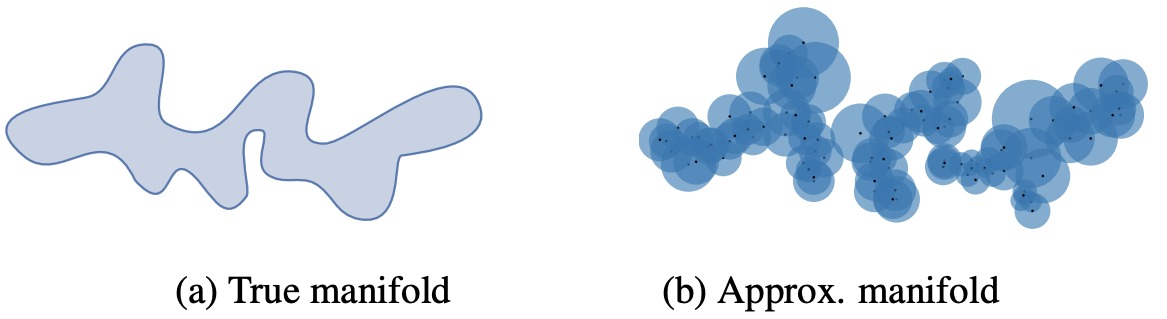
\includegraphics[width=0.75\linewidth]{figs/pr_k_nearest}
	\end{figure}
	\vspace{-0.3cm}
	The samples are embedded using a pretrained network, as in FID evaluation.
	\myfootnotewithlink{https://arxiv.org/abs/1904.06991}{Kynkäänniemi T. et al. Improved precision and recall metric for assessing generative models, 2019}
\end{frame}
%=======
\begin{frame}{Recap of Previous Lecture}
	\vspace{-0.2cm}
	\begin{minipage}{0.5\linewidth}
		\begin{block}{Unconditional Model}
			\begin{figure}
				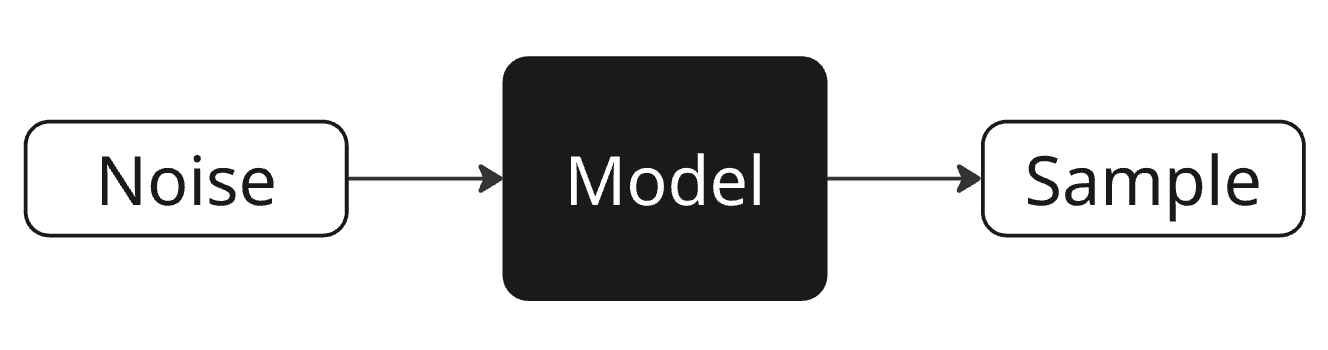
\includegraphics[width=0.95\linewidth]{figs/uncond_model}
			\end{figure}
		\end{block}
	\end{minipage}%
	\begin{minipage}{0.5\linewidth}
		\vspace{0.2cm}
		\begin{block}{Conditional Model}
			\begin{figure}
				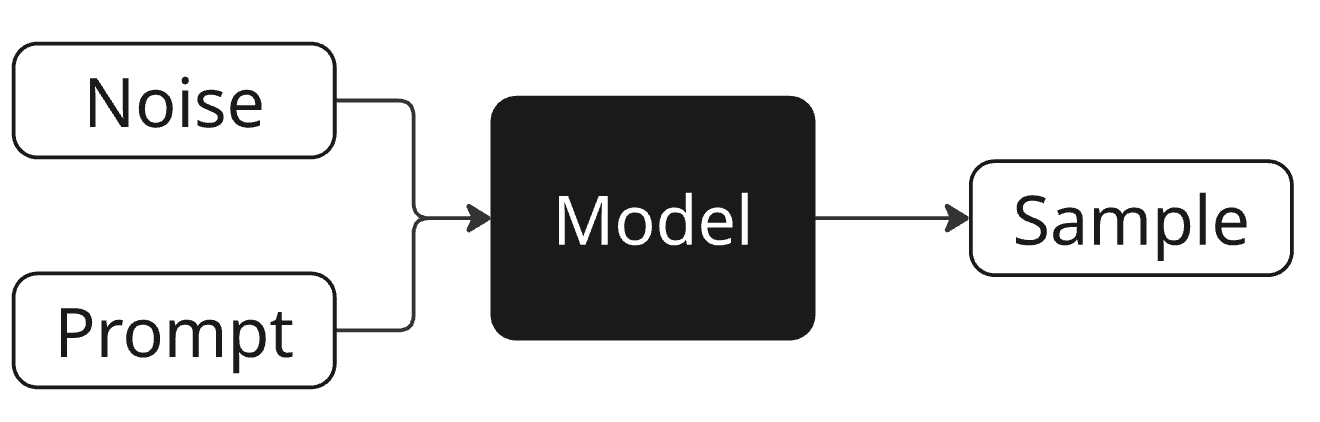
\includegraphics[width=0.95\linewidth]{figs/cond_model}
			\end{figure}
		\end{block}
	\end{minipage}
	We require metrics that evaluate not only the quality of generated images, but also their relevance to the prompt.
	\begin{block}{CLIP Score}
		\begin{figure}
			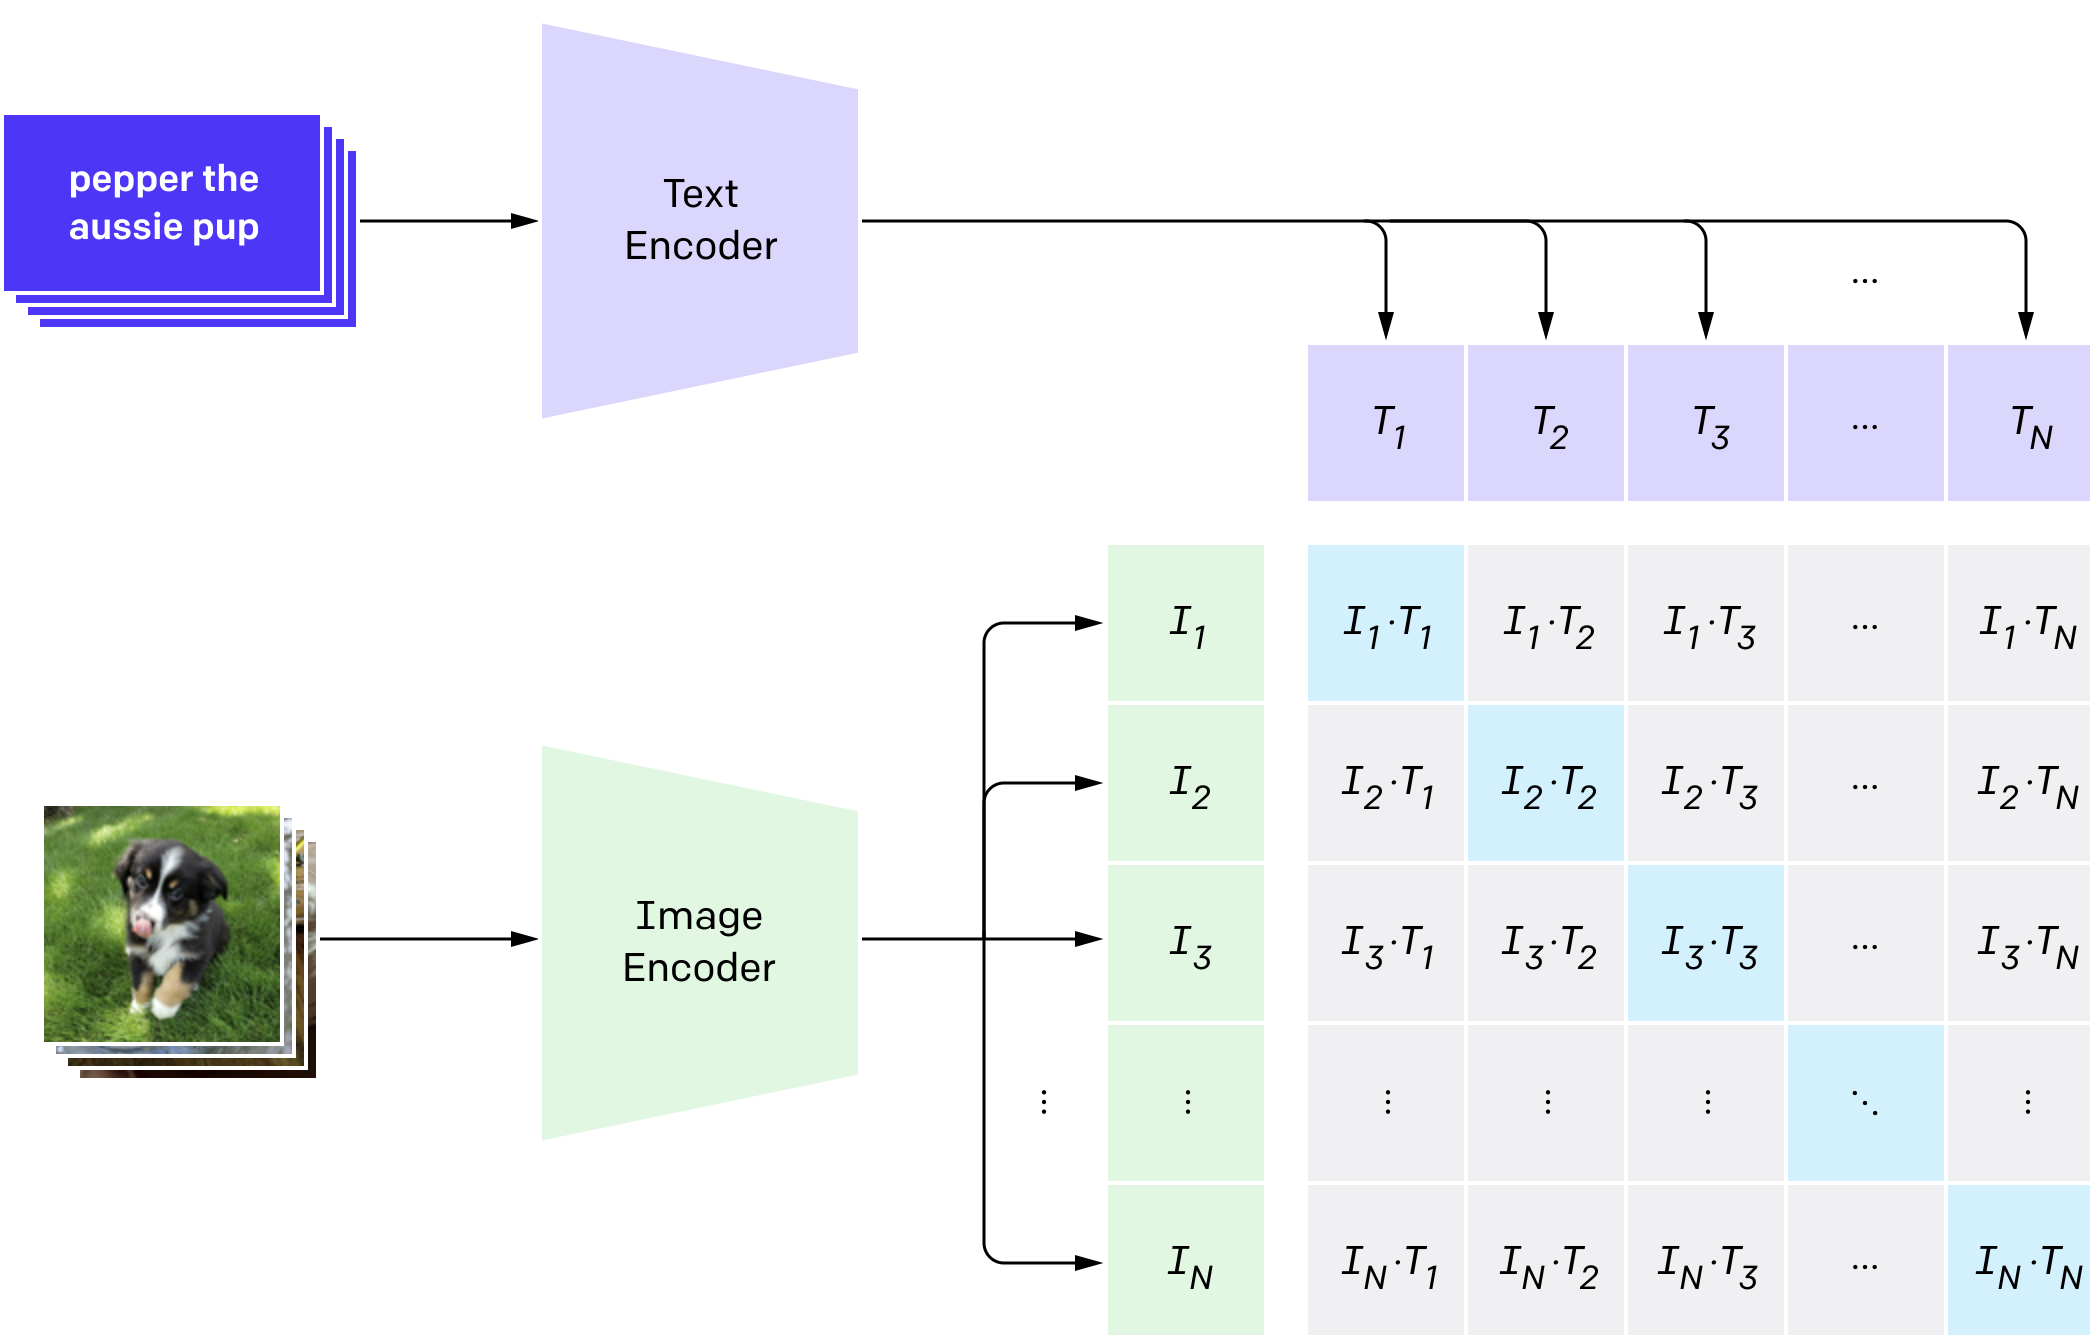
\includegraphics[width=0.5\linewidth]{figs/clip}
		\end{figure}
	\end{block}
	\myfootnotewithlink{https://arxiv.org/pdf/2103.00020}{Radford A. et al. Learning transferable visual models from natural language supervision, 2021} 
\end{frame}
%=======
\begin{frame}{Recap of Previous Lecture}
	\begin{itemize}
		\item No perfect automatic evaluation metric exists
		\item The most reliable assessment is via human evaluation
		\item It's important to evaluate a variety of model aspects
	\end{itemize}
	\begin{block}{Human Evaluation}
		\begin{figure}
			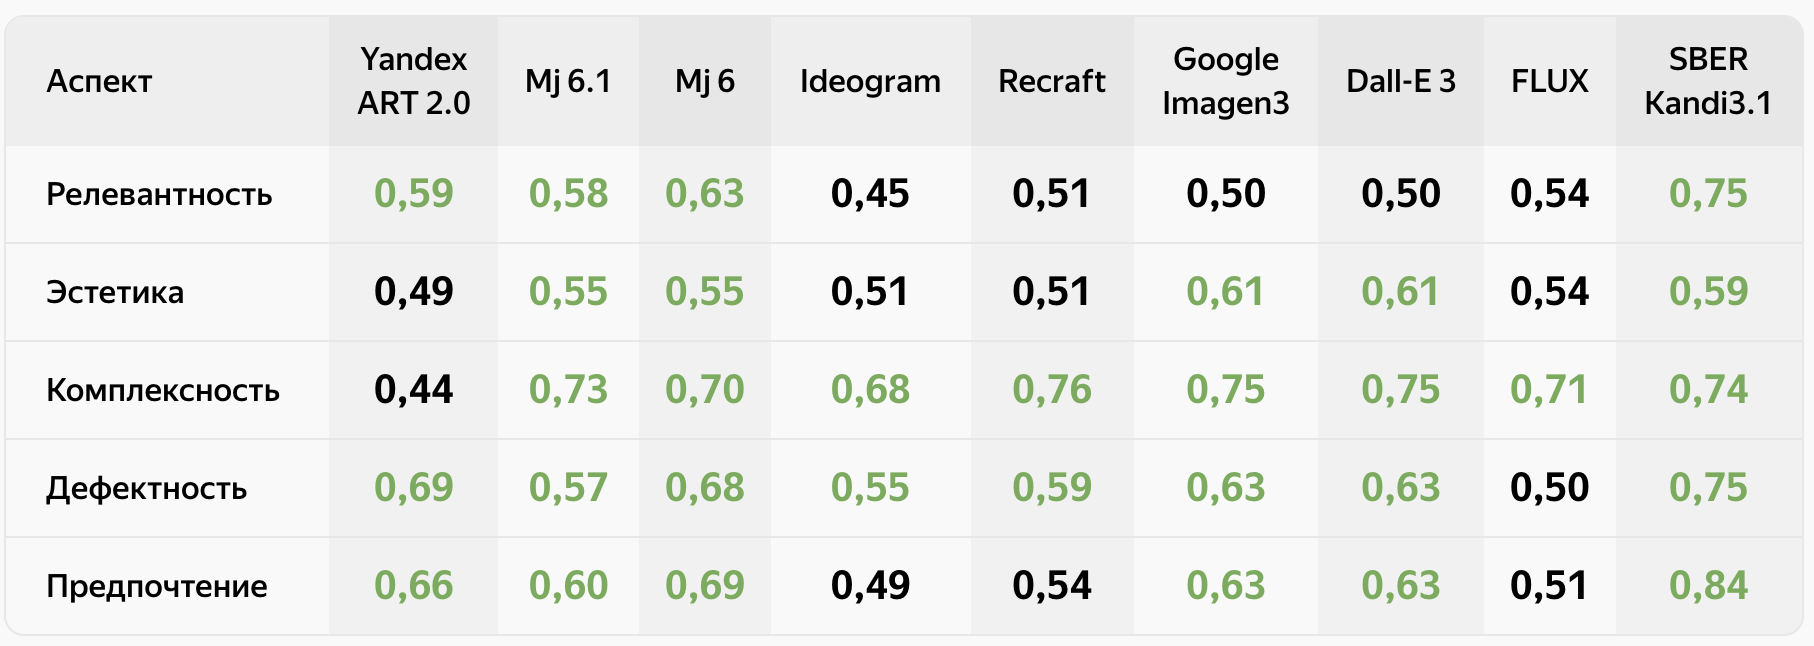
\includegraphics[width=1.0\linewidth]{figs/yaart_2.5}
		\end{figure}
	\end{block}
	\myfootnotewithlink{https://ya.ru/ai/art}{YandexART 2.5, 2025} 
\end{frame}
%=======
\begin{frame}{Recap of Previous Lecture}
	\begin{block}{Langevin Dynamics}
		\vspace{-0.3cm}
		\[
			\bx_{l + 1} = \bx_l + \frac{\eta}{2} \cdot \nabla_{\bx_l} \log p(\bx_l | \btheta) + \sqrt{\eta} \cdot \bepsilon_l, \quad \bepsilon_l \sim \cN(0, \bI)
		\]
		\vspace{-0.7cm}
	\end{block}
	\begin{block}{Fisher Divergence}
		\vspace{-0.3cm}
		\[
			D_F(\pi, p) = \frac{1}{2}\bbE_{\pi}\left\| \nabla_{\bx}\log p(\bx| \btheta) - \nabla_\bx \log \pi(\bx) \right\|_2^2 \rightarrow \min_{\btheta}
		\]
		\vspace{-0.7cm}
	\end{block}
	\begin{block}{Score Function}
		\vspace{-0.5cm}
		 \[
			 \bs_{\btheta}(\bx) = \nabla_{\bx}\log p(\bx| \btheta)
		 \]
	 \vspace{-0.8cm}
	\end{block}
	\begin{figure}
		\centering
		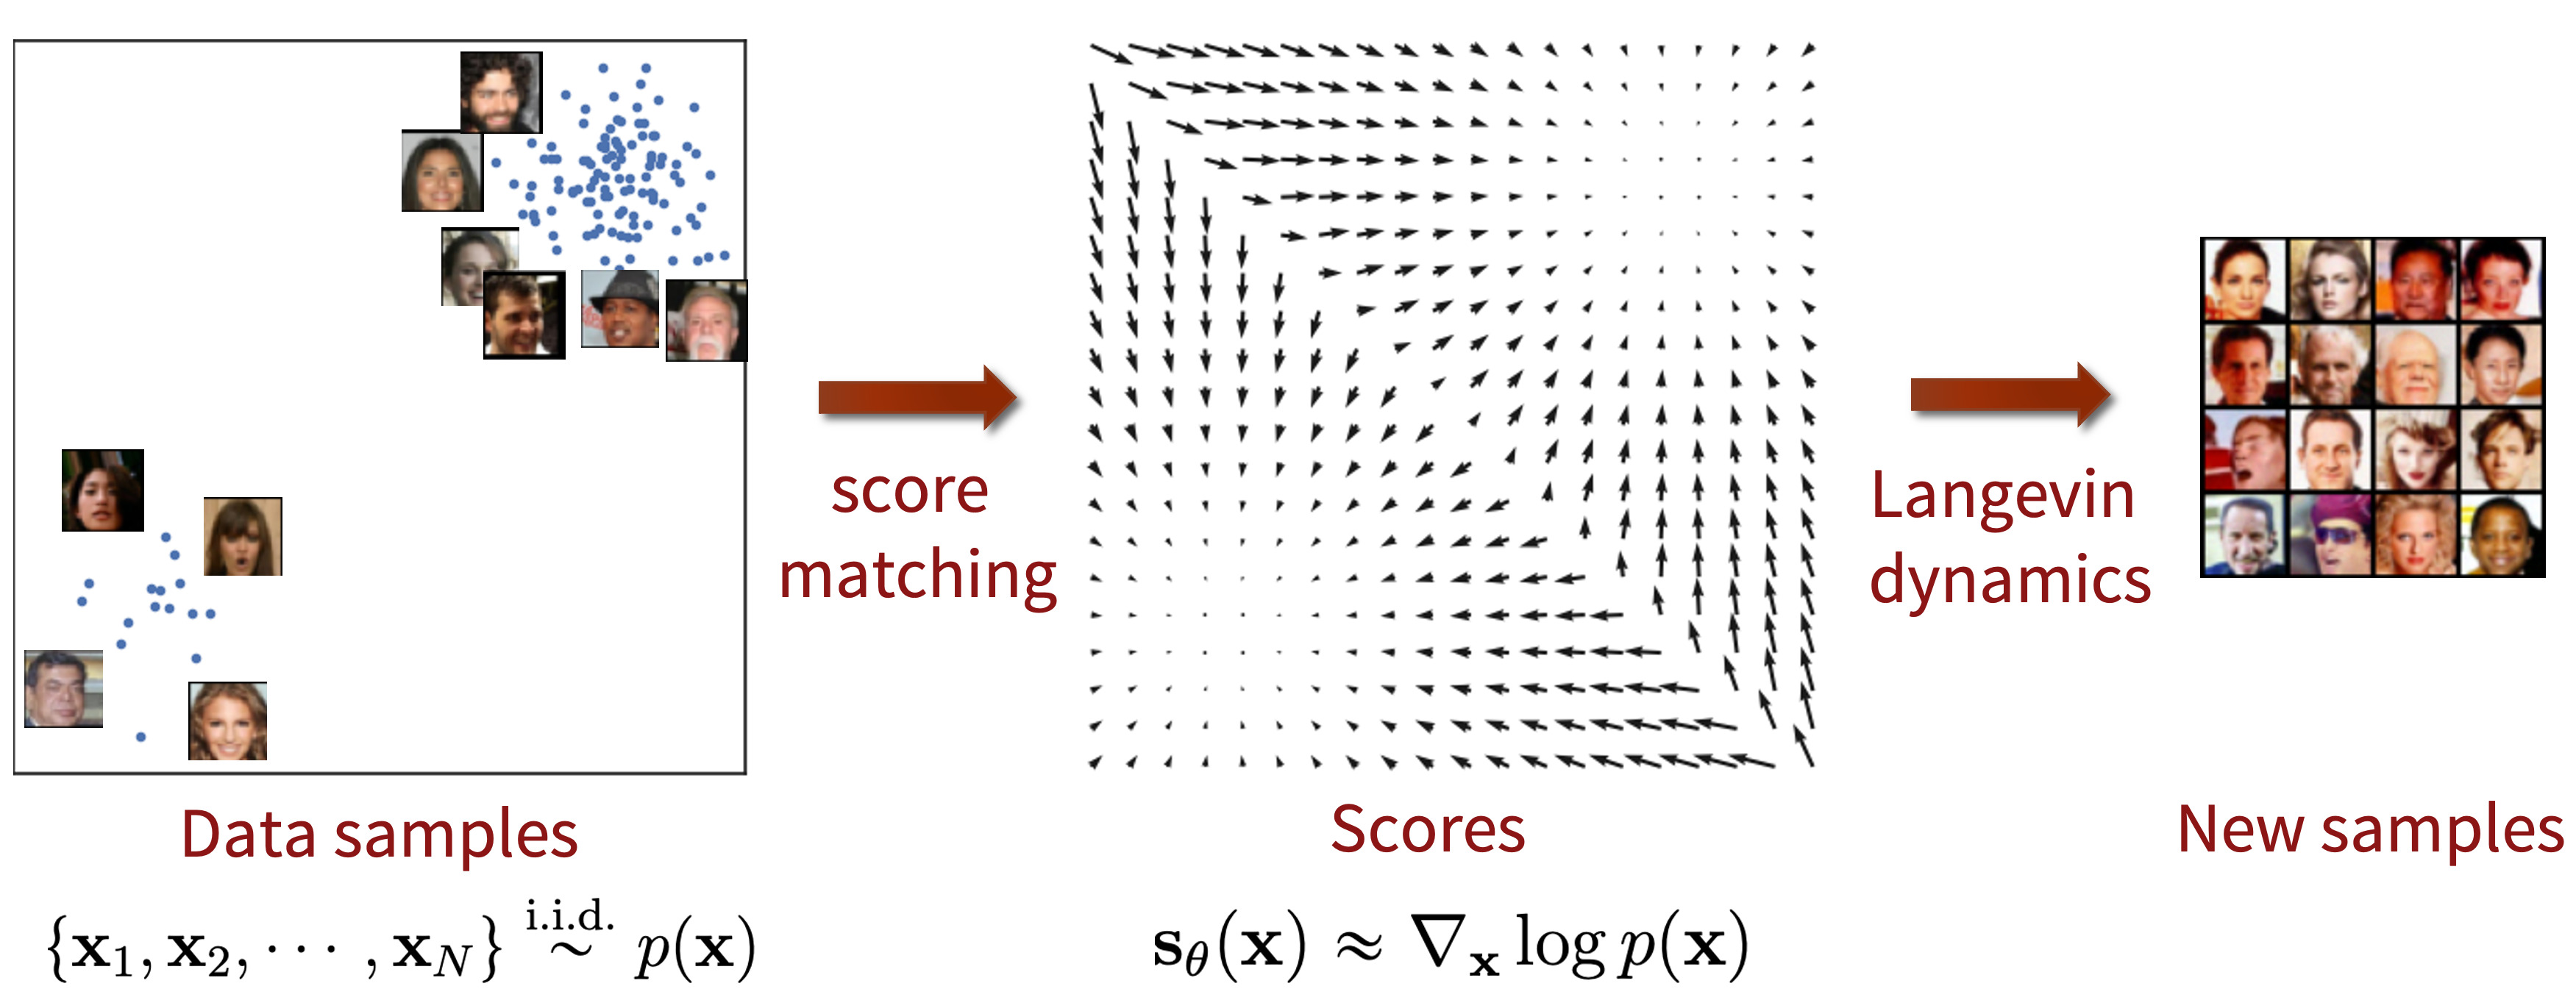
\includegraphics[width=0.75\linewidth]{figs/smld}
	\end{figure}
	\myfootnotewithlink{https://yang-song.github.io/blog/2021/score/}{Song Y. Generative Modeling by Estimating Gradients of the Data Distribution, blog post, 2021}
\end{frame}
%=======
\begin{frame}{Outline}
	\tableofcontents
\end{frame}
%=======
\section{Score Matching}
%=======
\subsection{Denoising Score Matching}
%=======
\begin{frame}{Denoising Score Matching}
	Let us perturb the original data $\bx \sim \pi(\bx)$ by adding Gaussian noise:
	\[
		\bx_{\sigma} = \bx + \sigma \bepsilon, \quad \bepsilon \sim \cN(0, \bI), \quad q(\bx_{\sigma} | \bx) = \cN(\bx, \sigma^2 \bI)
	\]
	\vspace{-0.4cm}
	\[
		q(\bx_{\sigma}) = \int q(\bx_{\sigma} | \bx) \pi(\bx) d\bx
	\]
	\vspace{-0.5cm} 
	\begin{block}{Assumption}
		The solution to
		\[
			\frac{1}{2} \bbE_{q(\bx_{\sigma})}\left\| \bs_{\btheta, \sigma}(\bx_{\sigma}) - \nabla_{\bx_{\sigma}} \log q(\bx_{\sigma}) \right\|_2^2 \rightarrow \min_{\btheta}
		\]
		\vspace{-0.3cm}
		satisfies $\bs_{\btheta, \sigma}(\bx_{\sigma}) \approx \bs_{\btheta, 0}(\bx_0) = \bs_{\btheta}(\bx)$ if $\sigma$ is sufficiently small.
	\end{block}
	\begin{itemize}
		\item The score function of the corrupted data closely approximates that of the original data
		\item The score function $\bs_{\btheta, \sigma}(\bx_{\sigma})$ is parameterized by $\sigma$
		\item \textbf{Note:} Neither $q(\bx_{\sigma})$ nor $\pi(\bx)$ are tractable
	\end{itemize}
	\myfootnotewithlink{http://www.iro.umontreal.ca/~vincentp/Publications/smdae_techreport.pdf}{Vincent P. A Connection Between Score Matching and Denoising Autoencoders, 2010}
\end{frame}
%=======
\begin{frame}{Denoising Score Matching}
	\begin{block}{Theorem}
	\vspace{-0.5cm}
	\begin{multline*}
		\bbE_{q(\bx_{\sigma})}\left\| \bs_{\btheta, \sigma}(\bx_{\sigma}) - \nabla_{\bx_{\sigma}} \log q(\bx_{\sigma}) \right\|_2^2 = \\
		= \bbE_{\pi(\bx)} \bbE_{q(\bx_{\sigma} | \bx)}\left\| \bs_{\btheta, \sigma}(\bx_{\sigma}) - \nabla_{\bx_{\sigma}} \log q(\bx_{\sigma} | \bx) \right\|_2^2 + \text{const}(\btheta)
	\end{multline*}
	\vspace{-0.5cm}
	\end{block}
	\begin{block}{Gradient of the Noise Kernel}
		\vspace{-0.3cm}
		\[
			\bx_{\sigma} = \bx + \sigma \bepsilon, \quad q(\bx_{\sigma} | \bx) = \cN(\bx, \sigma^2 \bI)
		\]
		\vspace{-0.3cm}
		\[
			\nabla_{\bx_{\sigma}} \log q(\bx_{\sigma} | \bx) = - \frac{\bx_{\sigma} - \bx}{\sigma^2}  = - \frac{\bepsilon}{\sigma}
		\]
		\vspace{-0.5cm}
	\end{block}
	\begin{itemize}
		\item The right-hand side does not require evaluating $\nabla_{\bx_{\sigma}} \log q(\bx_{\sigma})$ or $\nabla_{\bx_{\sigma}} \log \pi(\bx_{\sigma})$
		\item The neural network $\bs_{\btheta, \sigma}(\bx_{\sigma})$ is trained to \textbf{denoise} the corrupted samples $\bx_{\sigma}$
	\end{itemize}
	\myfootnotewithlink{http://www.iro.umontreal.ca/~vincentp/Publications/smdae_techreport.pdf}{Vincent P. A Connection Between Score Matching and Denoising Autoencoders, 2010}
\end{frame}
%=======
\begin{frame}{Denoising Score Matching}
	\begin{block}{Theorem}
	\vspace{-0.5cm}
	\begin{multline*}
		\bbE_{q(\bx_{\sigma})}\underbrace{\left\| \bs_{\btheta, \sigma}(\bx_{\sigma}) - \nabla_{\bx_{\sigma}} \log q(\bx_{\sigma}) \right\|_2^2}_{h(\bx_{\sigma})} = \\
		= \bbE_{\pi(\bx)} \bbE_{q(\bx_{\sigma} | \bx)}\left\| \bs_{\btheta, \sigma}(\bx_{\sigma}) - \nabla_{\bx_{\sigma}} \log q(\bx_{\sigma} | \bx) \right\|_2^2 + \text{const}(\btheta)
	\end{multline*}
	\vspace{-0.5cm}
	\end{block}
	\begin{block}{Proof}
		\vspace{-0.7cm}
		\begin{multline*}
			\bbE_{q(\bx_{\sigma})} h(\bx_{\sigma}) = \int {\color{violet}q(\bx_{\sigma})} h(\bx_{\sigma}) d\bx_{\sigma} = \\
			= \int \left({\color{violet}\int q(\bx_{\sigma} | \bx) \pi(\bx) d\bx}\right) h(\bx_{\sigma}) d\bx_{\sigma} =  \bbE_{\pi(\bx)} \bbE_{q(\bx_{\sigma} | \bx)}  h(\bx_{\sigma})
		\end{multline*}
		\vspace{-0.7cm}
		{\small
		\begin{multline*}
			\bbE_{q(\bx_{\sigma})}\left\| \bs_{\btheta, \sigma}(\bx_{\sigma}) - \nabla_{\bx_{\sigma}} \log q(\bx_{\sigma}) \right\|_2^2 = \\ 
			= \bbE_{q(\bx_{\sigma})} \Bigl[\| \bs_{\btheta, \sigma}(\bx_{\sigma}) \|^2 + \underbrace{\| \nabla_{\bx_{\sigma}} \log q(\bx_{\sigma}) \|_2^2}_{\text{const}(\btheta)} - 2 {\color{teal}\bs_{\btheta, \sigma}^T(\bx_{\sigma}) \nabla_{\bx_{\sigma}} \log q(\bx_{\sigma})} \Bigr]
		\end{multline*}
		}
	\end{block}
	\myfootnotewithlink{http://www.iro.umontreal.ca/~vincentp/Publications/smdae_techreport.pdf}{Vincent P. A Connection Between Score Matching and Denoising Autoencoders, 2010}
\end{frame}
%=======
\begin{frame}{Denoising Score Matching}
	\begin{block}{Theorem}
	\vspace{-0.5cm}
	\begin{multline*}
		\bbE_{q(\bx_{\sigma})}\left\| \bs_{\btheta, \sigma}(\bx_{\sigma}) - \nabla_{\bx_{\sigma}} \log q(\bx_{\sigma}) \right\|_2^2 = \\
		= \bbE_{\pi(\bx)} \bbE_{q(\bx_{\sigma} | \bx)}\left\| \bs_{\btheta, \sigma}(\bx_{\sigma}) - \nabla_{\bx_{\sigma}} \log q(\bx_{\sigma} | \bx) \right\|_2^2 + \text{const}(\btheta)
	\end{multline*}
	\vspace{-0.5cm}
	\end{block}
	\begin{block}{Proof (Continued)}
		\vspace{-0.7cm}
		{\small
		\begin{multline*}
			\bbE_{q(\bx_{\sigma})} \left[{\color{teal}\bs_{\btheta, \sigma}^T(\bx_{\sigma}) \nabla_{\bx_{\sigma}} \log q(\bx_{\sigma})} \right] = \int q(\bx_{\sigma}) \left[\bs_{\btheta, \sigma}^T(\bx_{\sigma}) \frac{\nabla_{\bx_{\sigma}} {\color{violet}q(\bx_{\sigma})}}{q(\bx_{\sigma})} \right] d\bx_{\sigma} = \\
			= \int \left[\bs_{\btheta, \sigma}^T(\bx_{\sigma}) \nabla_{\bx_{\sigma}}\left({\color{violet}\int q(\bx_{\sigma} | \bx) \pi(\bx) d\bx}\right) \right] d\bx_{\sigma} = \\
			=  \int \int \pi(\bx) \left[\bs_{\btheta, \sigma}^T(\bx_{\sigma}) {\color{olive}\nabla_{\bx_{\sigma}}q(\bx_{\sigma} | \bx)} \right] d\bx_{\sigma} d\bx = \\
			= \int \int \pi(\bx) {\color{olive} q(\bx_{\sigma} | \bx)} \left[\bs_{\btheta, \sigma}^T(\bx_{\sigma}) {\color{olive}\nabla_{\bx_{\sigma}} \log q(\bx_{\sigma} | \bx)} \right] d\bx_{\sigma} d\bx = \\
			= \bbE_{\pi(\bx)} \bbE_{q(\bx_{\sigma} | \bx)} \left[{\color{teal}\bs_{\btheta, \sigma}^T(\bx_{\sigma}) \nabla_{\bx_{\sigma}} \log q(\bx_{\sigma} | \bx)} \right]
		\end{multline*}
		}
	\end{block}
	\myfootnotewithlink{http://www.iro.umontreal.ca/~vincentp/Publications/smdae_techreport.pdf}{Vincent P. A Connection Between Score Matching and Denoising Autoencoders, 2010}
\end{frame}
%=======
\begin{frame}{Denoising Score Matching}
	\vspace{-0.3cm}
	\begin{block}{Theorem}
	\vspace{-0.7cm}
	\begin{multline*}
		\bbE_{q(\bx_{\sigma})}\underbrace{\left\| \bs_{\btheta, \sigma}(\bx_{\sigma}) - \nabla_{\bx_{\sigma}} \log q(\bx_{\sigma}) \right\|_2^2}_{h(\bx_{\sigma})} = \\
		= \bbE_{\pi(\bx)} \bbE_{q(\bx_{\sigma} | \bx)}\left\| \bs_{\btheta, \sigma}(\bx_{\sigma}) - \nabla_{\bx_{\sigma}} \log q(\bx_{\sigma} | \bx) \right\|_2^2 + \text{const}(\btheta)
	\end{multline*}
	\vspace{-0.9cm}
	\end{block}
	\begin{block}{Proof (Continued)}
		\vspace{-0.3cm}
		\[
			\bbE_{q(\bx_{\sigma})} h(\bx_{\sigma})=  \bbE_{\pi(\bx)} \bbE_{q(\bx_{\sigma} | \bx)}  h(\bx_{\sigma})
		\]
		\[
			\bbE_{q(\bx_{\sigma})} \left[\bs_{\btheta, \sigma}^T(\bx_{\sigma}) \nabla_{\bx_{\sigma}} \log q(\bx_{\sigma}) \right] = \bbE_{\pi(\bx)} \bbE_{q(\bx_{\sigma} | \bx)} \left[\bs_{\btheta, \sigma}^T(\bx_{\sigma}) \nabla_{\bx_{\sigma}} \log q(\bx_{\sigma} | \bx) \right]
		\]
		\vspace{-0.5cm}
		{\small
		\begin{multline*}
			\bbE_{q(\bx_{\sigma})}\left\| \bs_{\btheta, \sigma}(\bx_{\sigma}) - \nabla_{\bx_{\sigma}} \log q(\bx_{\sigma}) \right\|_2^2 = \\ 
			= {\color{olive}\bbE_{\pi(\bx)} \bbE_{q(\bx_{\sigma} | \bx)}}\left[\| \bs_{\btheta, \sigma}(\bx_{\sigma}) \|^2 - 2 \bs_{\btheta, \sigma}^T(\bx_{\sigma}) {\color{teal}\nabla_{\bx_{\sigma}} \log q(\bx_{\sigma} | \bx)} \right] + \text{const}(\btheta) \\
			= {\color{olive}\bbE_{\pi(\bx)} \bbE_{q(\bx_{\sigma} | \bx)}} \left\|\bs_{\btheta, \sigma}(\bx_{\sigma}) - {\color{teal}\nabla_{\bx_{\sigma}} \log q(\bx_{\sigma} | \bx)} \right\|_2^2 + \text{const}(\btheta)
		\end{multline*}
		}
		\vspace{-0.8cm}
	\end{block}
	\myfootnotewithlink{http://www.iro.umontreal.ca/~vincentp/Publications/smdae_techreport.pdf}{Vincent P. A Connection Between Score Matching and Denoising Autoencoders, 2010}
\end{frame}
%=======
\begin{frame}{Denoising Score Matching}
	Original objective:
	\vspace{-0.2cm}
	\[
		\bbE_{\pi(\bx)}\left\| \bs_{\btheta}(\bx) - \nabla_\bx \log \pi(\bx) \right\|_2^2 \rightarrow \min_{\btheta}
	\]
	\vspace{-0.5cm} \\
	Noisy objective:
	\vspace{-0.2cm}
	\[
		\bbE_{q(\bx_{\sigma})}\left\| \bs_{\btheta, \sigma}(\bx_\sigma) - \nabla_\bx \log q(\bx_{\sigma}) \right\|_2^2 \rightarrow \min_{\btheta}
	\]
	\vspace{-0.5cm} \\
	This is equivalent to a denoising task:
	\vspace{-0.2cm}
	\[
		\bbE_{\pi(\bx)} \bbE_{q(\bx_{\sigma} | \bx)}\left\| \bs_{\btheta, \sigma}(\bx_{\sigma}) - \nabla_{\bx_{\sigma}} \log q(\bx_{\sigma} | \bx) \right\|_2^2 \rightarrow \min_{\btheta}
	\]
	\vspace{-0.3cm}
	\[
		\bbE_{\pi(\bx)} \bbE_{\cN(0, \bI)}\left\| \bs_{\btheta, \sigma}(\bx + \sigma \bepsilon) + \frac{\bepsilon}{\sigma} \right\|_2^2 \rightarrow \min_{\btheta}
	\]
	\vspace{-0.5cm}
	\begin{block}{Langevin Dynamics}
		\vspace{-0.3cm}
		\[
			\bx_{l + 1} = \bx_l + \frac{\eta}{2} \cdot \bs_{\btheta, \sigma}(\bx_l) + \sqrt{\eta} \cdot \bepsilon_l, \quad \bepsilon_l \sim \cN(0, \bI)
		\]
		\vspace{-0.7cm}
	\end{block}
	\myfootnotewithlink{https://yang-song.github.io/blog/2021/score/}{Song Y. Generative Modeling by Estimating Gradients of the Data Distribution, blog post, 2021}
\end{frame}
%=======
\subsection{Noise-Conditioned Score Network}
%=======
\begin{frame}{Denoising Score Matching}
	\vspace{-0.5cm}
	\[
		\bbE_{\pi(\bx)} \bbE_{\cN(0, \bI)}\left\| \bs_{\btheta, \sigma}(\bx + \sigma \bepsilon) + \frac{\bepsilon}{\sigma} \right\|_2^2 \rightarrow \min_{\btheta}
	\]
	\begin{minipage}{0.5\linewidth}
		\[
			\bx_{l + 1} = \bx_l + \frac{\eta}{2} \cdot \bs_{\btheta, \sigma}(\bx_l) + \sqrt{\eta} \cdot \bepsilon_l
		\]
		\vspace{-0.3cm}
		\begin{itemize}
			\item For \textbf{small} $\sigma$, $\bs_{\btheta, \sigma}(\bx)$ becomes inaccurate and Langevin dynamics fails to traverse modes
			\item For \textbf{large} $\sigma$, robustness in low-density regions is achieved, but the model learns a distribution that is overly corrupted
		\end{itemize}
	\end{minipage}%
	\begin{minipage}{0.5\linewidth}
		\begin{figure}
			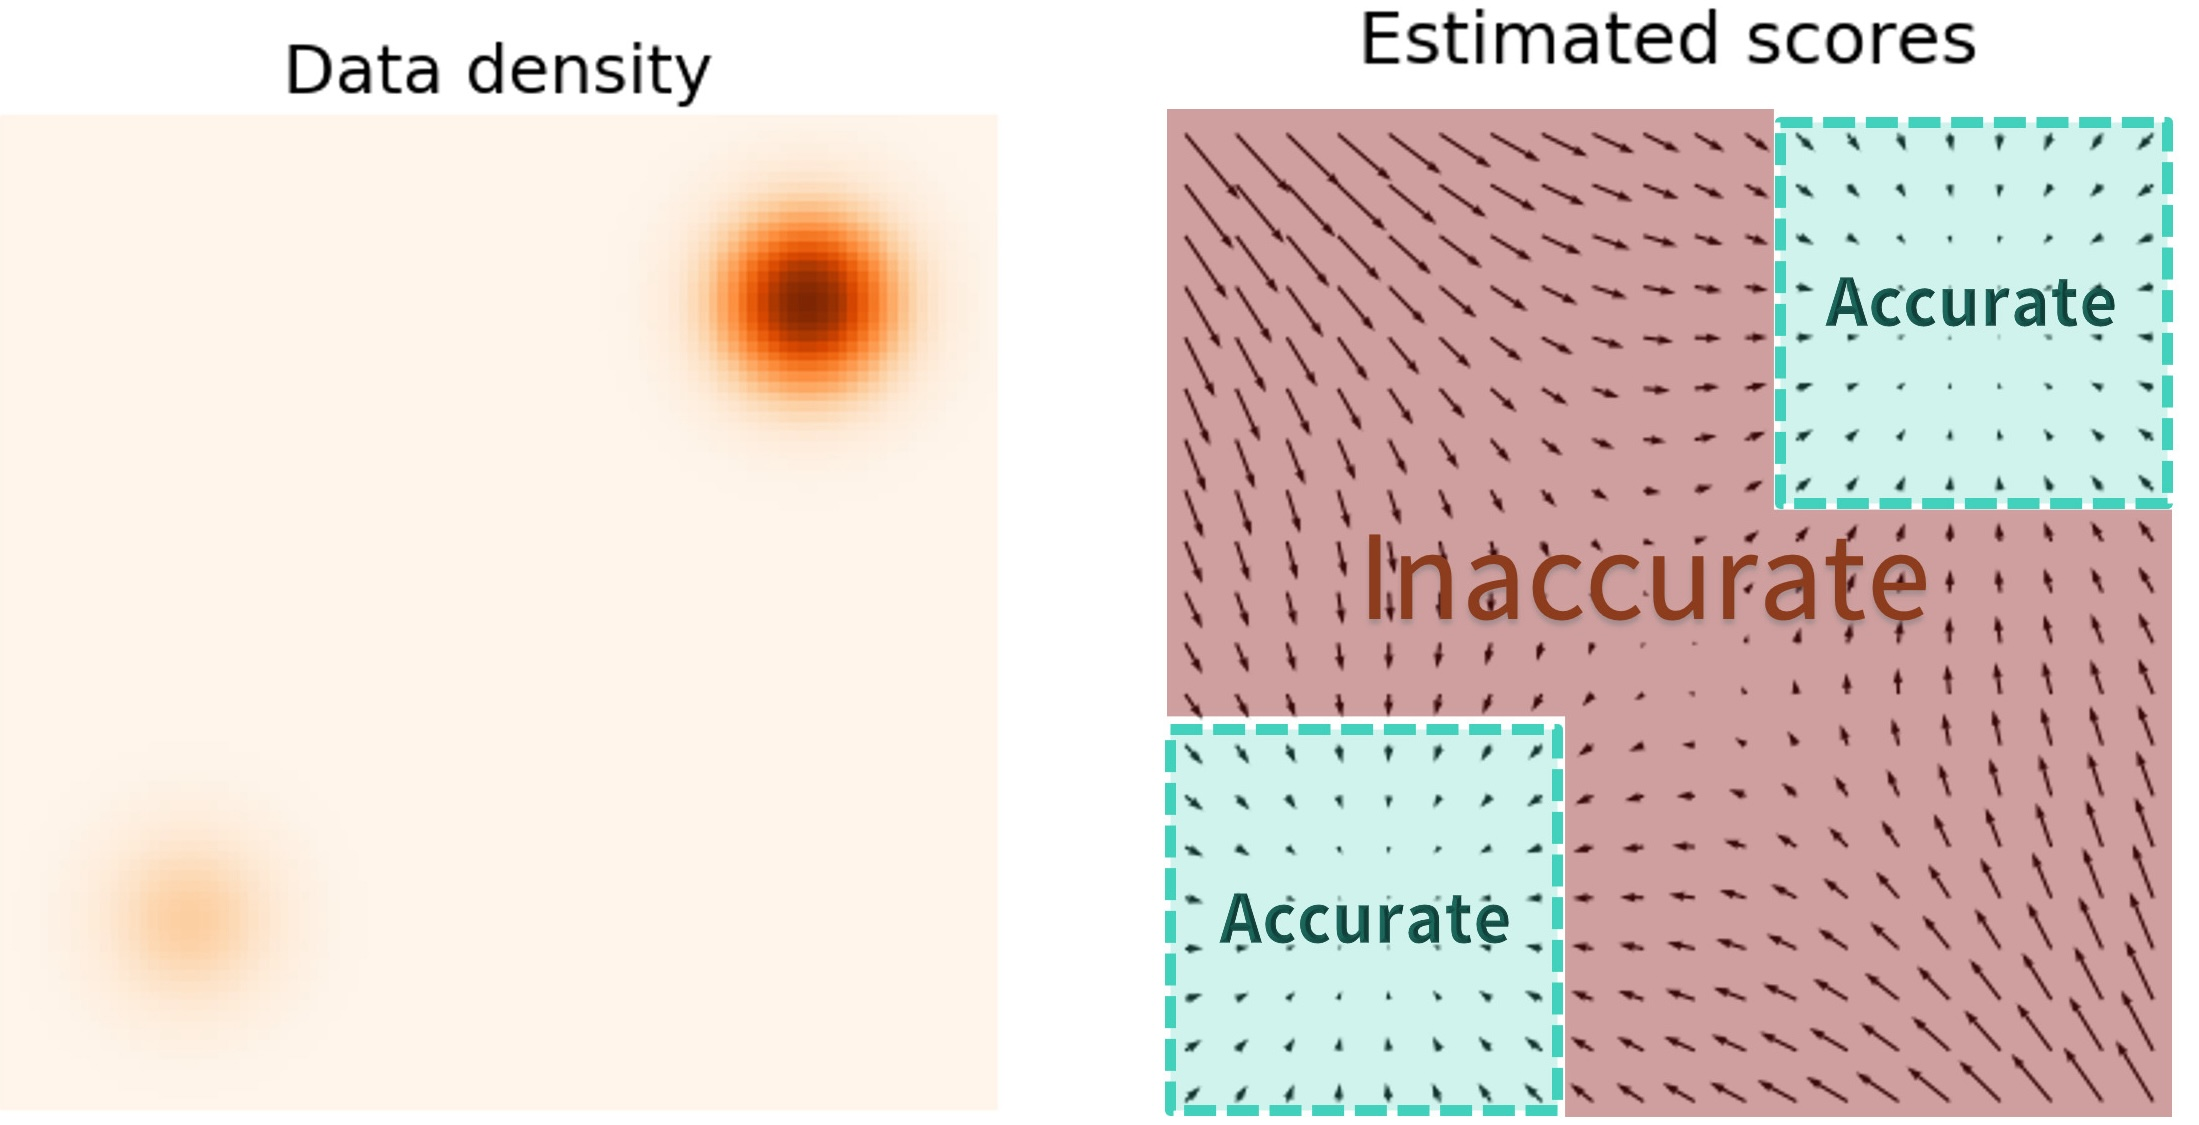
\includegraphics[width=\linewidth]{figs/pitfalls}
		\end{figure}
		\vspace{-0.3cm}
		\begin{figure}
			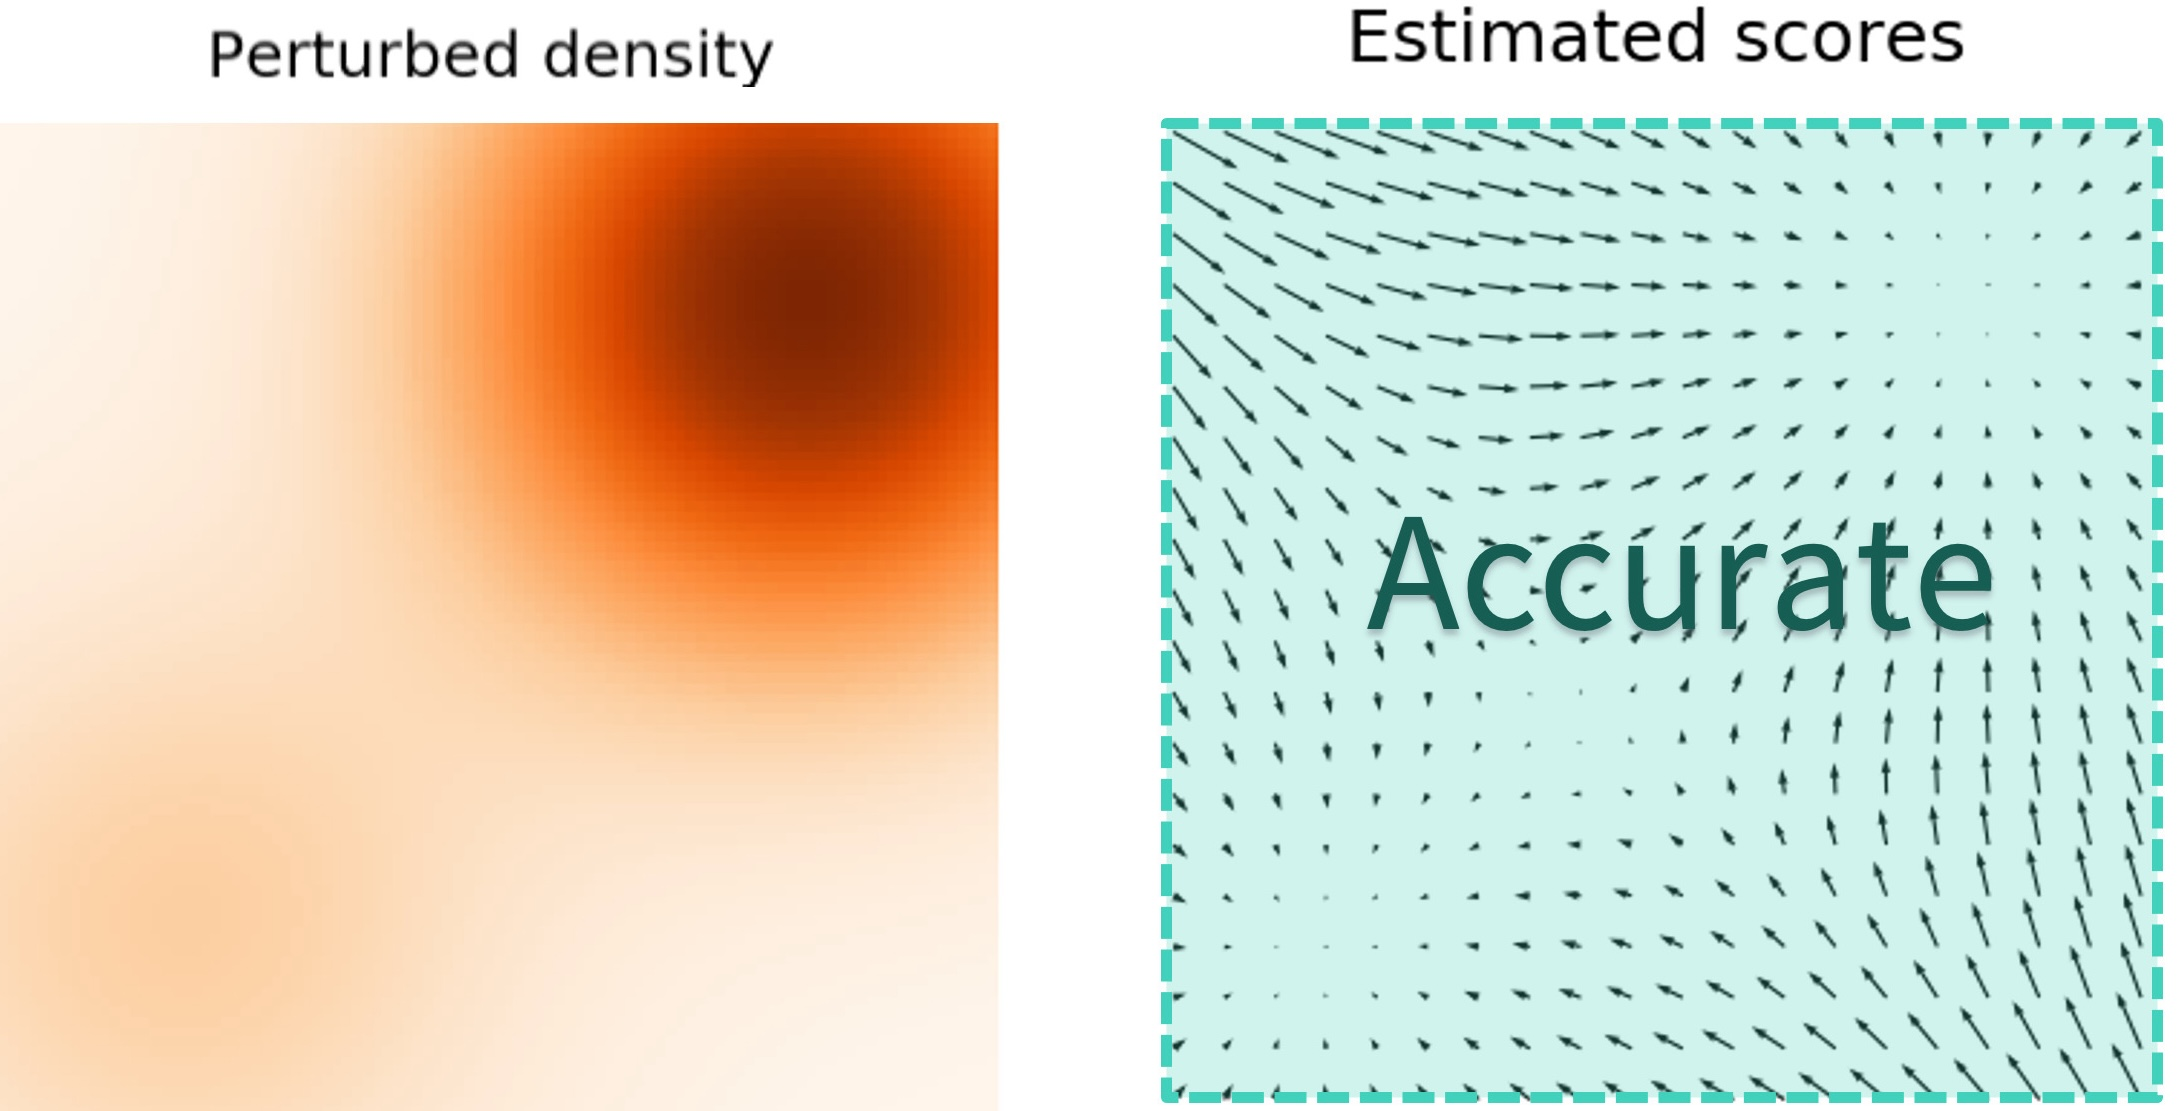
\includegraphics[width=\linewidth]{figs/single_noise}
		\end{figure}
	\end{minipage}
	\myfootnotewithlink{https://yang-song.github.io/blog/2021/score/}{Song Y. Generative Modeling by Estimating Gradients of the Data Distribution, blog post, 2021}
\end{frame}
%=======
\begin{frame}{Noise-Conditioned Score Network (NCSN)}
	\begin{itemize}
		\item Specify a sequence of noise levels: $\sigma_1 < \sigma_2 < \dots < \sigma_T$
		\item Perturb each data point with different noise levels: $\bx_t = \bx + \sigma_t \bepsilon$, so $\bx_t \sim q(\bx_t)$
		\item Choose $\sigma_1, \sigma_T$ such that:
		\[
			q(\bx_1) \approx \pi(\bx), \;\; q(\bx_T) \approx \cN(0, \sigma_T^2 \bI)
		\]
	\end{itemize}
	\begin{figure}
		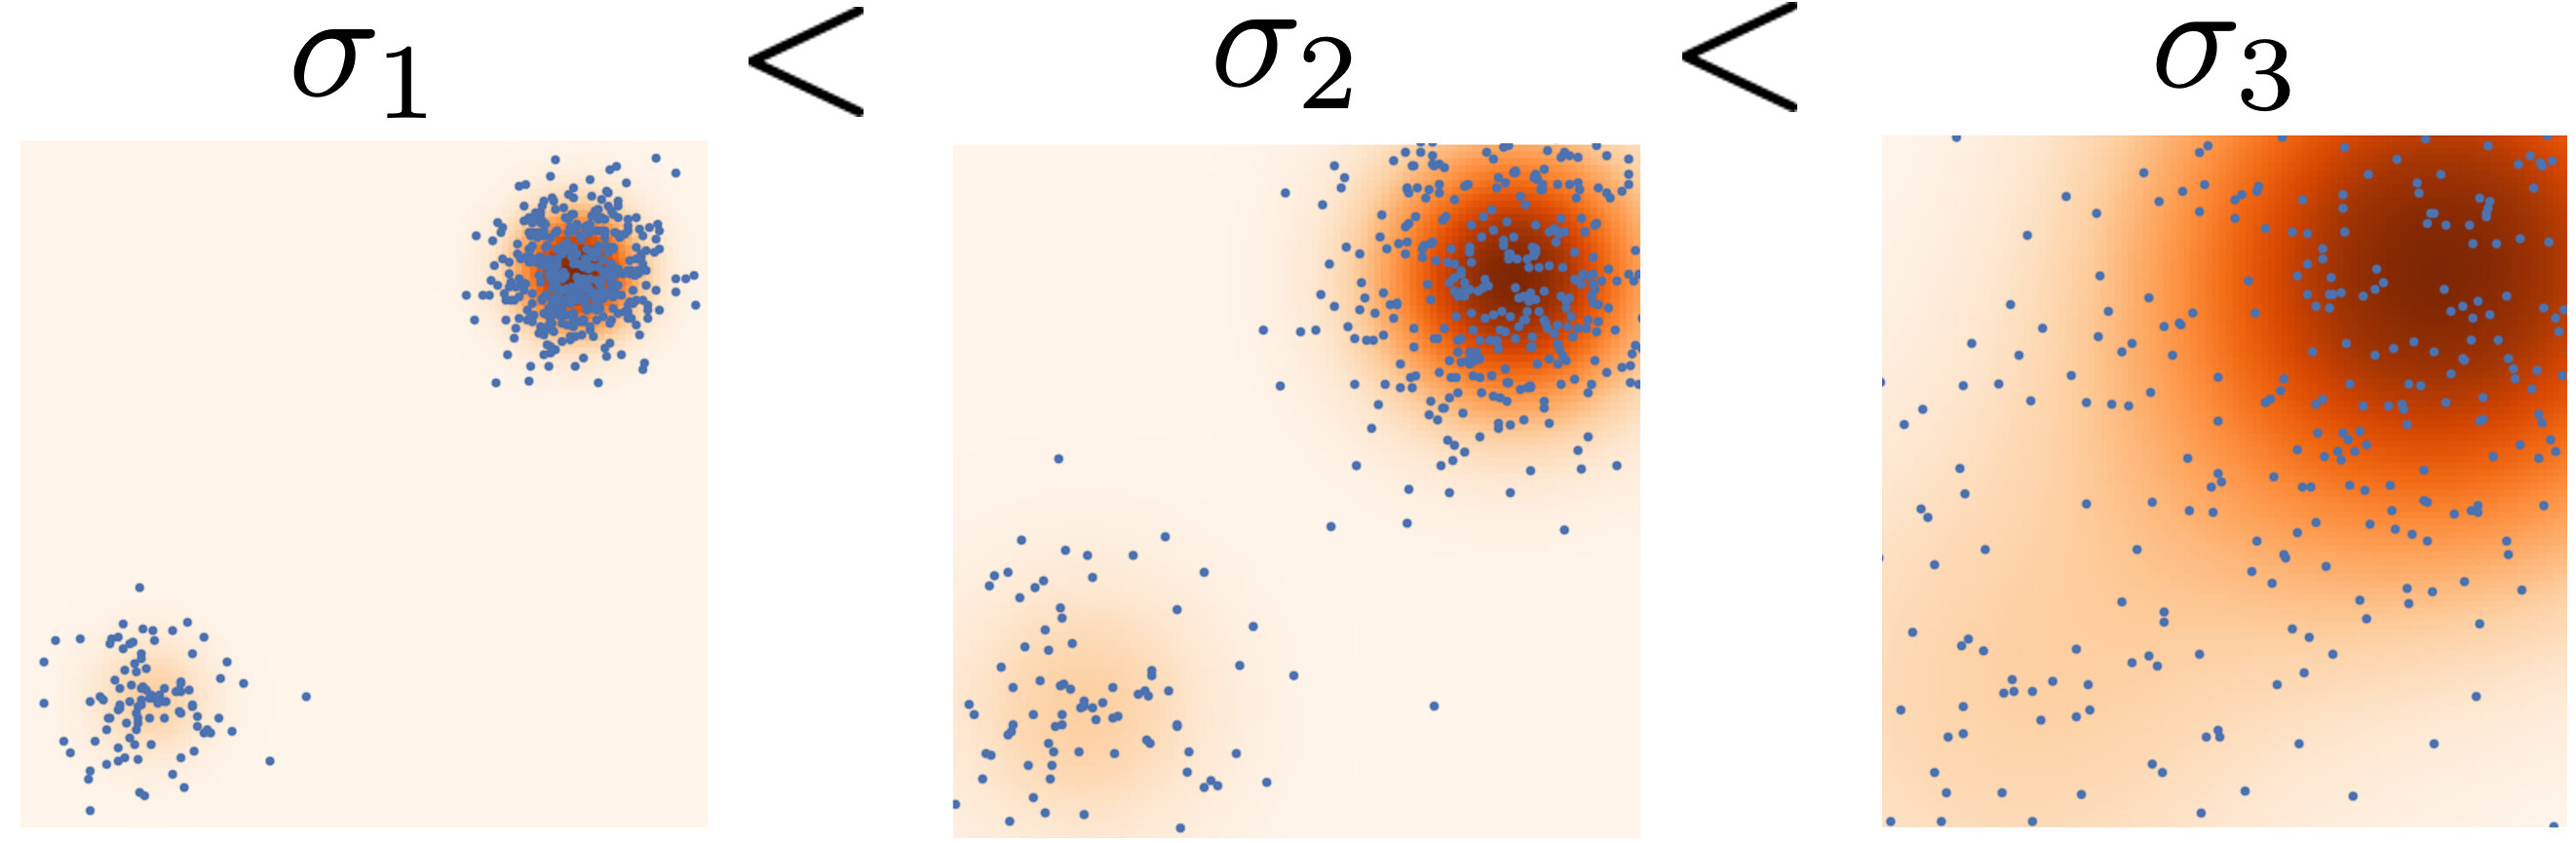
\includegraphics[width=0.6\linewidth]{figs/multi_scale}
	\end{figure}
	\begin{figure}
		
\includegraphics[width=\linewidth]{figs/duoduo}
	\end{figure}
	\myfootnotewithlink{https://arxiv.org/abs/1907.05600}{Song Y. et al. Generative Modeling by Estimating Gradients of the Data Distribution, 2019}
\end{frame}
%=======
\begin{frame}{Noise-Conditioned Score Network (NCSN)}
	Train the denoising score function $\bs_{\btheta, \sigma_t}(\bx_t)$ for each noise level $\sigma_t$ using a unified weighted objective:
	\vspace{-0.2cm}
	\[
		\sum_{t=1}^T {\color{violet}\sigma_t^2} \bbE_{\pi(\bx)} \bbE_{q(\bx_t | \bx)}\left\| \bs_{\btheta, \sigma_t}(\bx_t) - \nabla_{\bx_t} \log q(\bx_t | \bx) \right\|_2^2 \rightarrow \min_{\btheta}
	\]
	Here, $\nabla_{\bx_t} \log q(\bx_t | \bx) = - \frac{\bx_t - \bx}{\sigma_t^2} = - \frac{\bepsilon}{\sigma_t}$
	\begin{block}{Training Procedure}
		\begin{enumerate}
			\item Sample $\bx_0 \sim \pi(\bx)$
			\item Sample $t \sim U\{1, T\}$ and $\bepsilon \sim \cN(0, \bI)$
			\item Construct noisy image $\bx_t = \bx_0 + \sigma_t \bepsilon$
			\item Evaluate loss $ \cL = \sigma_t^2 \left\| \bs_{\btheta, \sigma_t}(\bx_t) + \frac{\bepsilon}{\sigma_t} \right\|^2 $
		\end{enumerate}
		\vspace{-0.3cm}
	\end{block}
	How do we sample from such a model?
	\myfootnotewithlink{https://arxiv.org/abs/1907.05600}{Song Y. et al. Generative Modeling by Estimating Gradients of the Data Distribution, 2019}
\end{frame}
%=======
\begin{frame}{Noise-Conditioned Score Network (NCSN)}
	\begin{block}{Sampling (Annealed Langevin Dynamics)}
		\begin{itemize}
			\item Sample initial point $\bx_0 \sim \cN(0, \sigma_T^2 \bI) \approx q(\bx_T)$
			\item At each noise level, apply $L$ steps of Langevin dynamics:
			\vspace{-0.2cm}
			\[
				\bx_l = \bx_{l-1} + \frac{\eta_t}{2} \bs_{\btheta, \sigma_t}(\bx_{l-1}) + \sqrt{\eta_t} \bepsilon_l,
			\] 
			\vspace{-0.5cm}
			\item Update $\bx_0 := \bx_L$ and reduce to the next lower $\sigma_t$
		\end{itemize}
	\end{block}
	\begin{figure}
		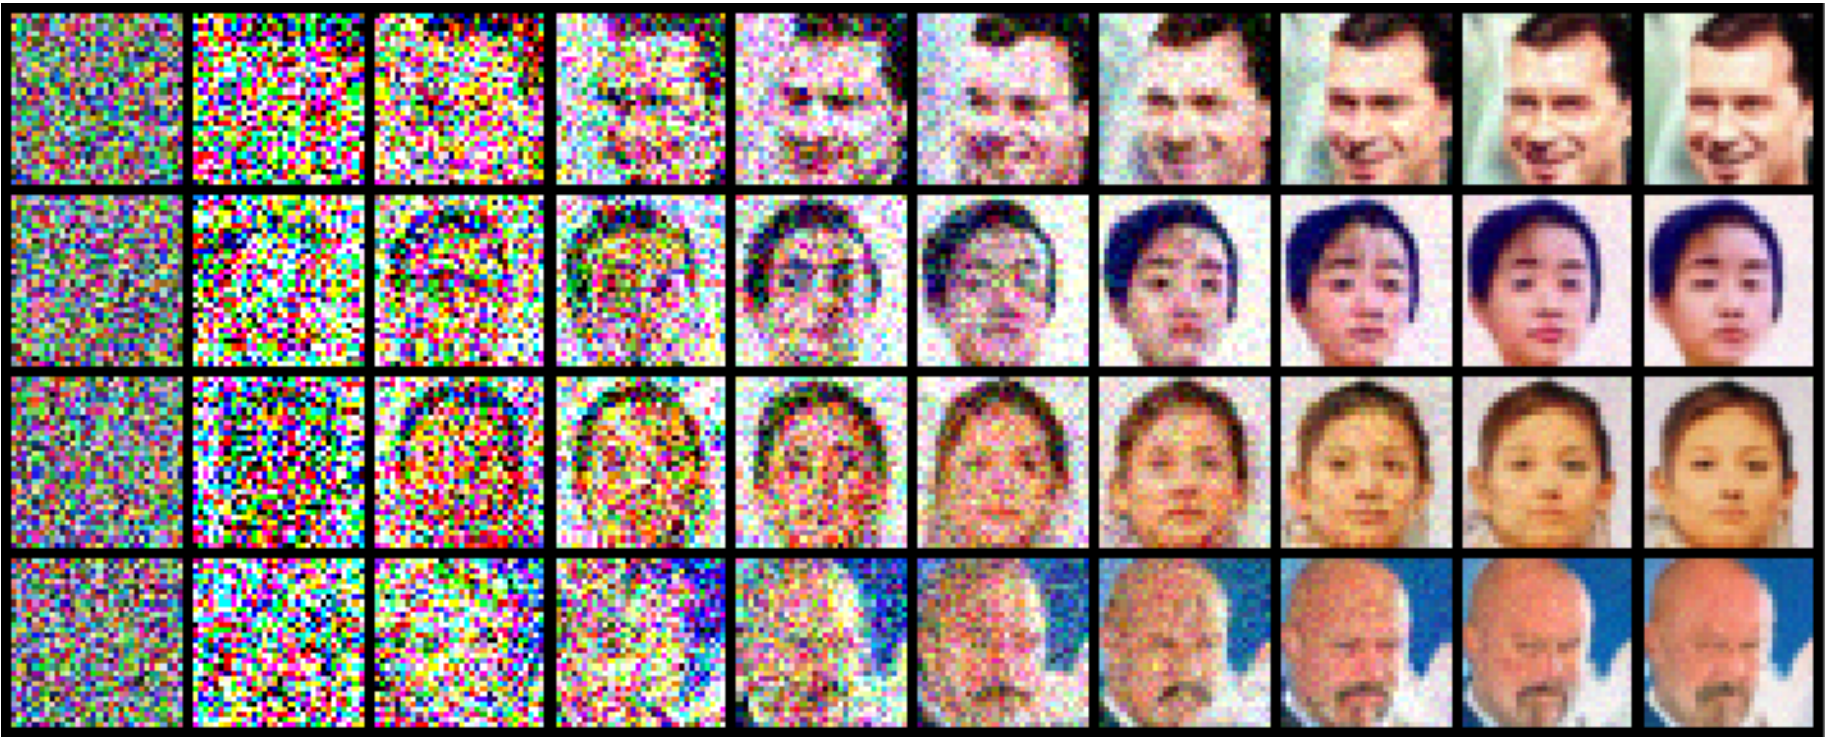
\includegraphics[width=0.9\linewidth]{figs/ald}
	\end{figure}
	\myfootnotewithlink{https://arxiv.org/abs/2006.09011}{Song Y. et al. Improved Techniques for Training Score-Based Generative Models, 2020}
\end{frame}
%=======
\section{Forward Gaussian Diffusion Process}
%=======
\begin{frame}{Forward Gaussian Diffusion Process}
	Let $\bx_0 = \bx \sim \pi(\bx)$, $\beta_t \ll 1$. Define a Markov chain:
	\[
		\bx_t = \sqrt{1 - \beta_t} \bx_{t-1} + \sqrt{\beta_t} \bepsilon_t, \;\; \bepsilon_t \sim \cN(0, \bI)
	\]
	\[
		q(\bx_t | \bx_{t-1}) = \cN(\sqrt{1 - \beta_t} \bx_{t-1}, \beta_t \bI)
	\]
	\vspace{-0.5cm}
	\begin{block}{Langevin Dynamics}
		\vspace{-0.3cm}
		\[
			\bx_{l + 1} = \bx_l + \frac{ \color{violet} \eta}{2} \cdot {\color{teal}\nabla_{\bx_l} \log p(\bx_l | \btheta)} + \sqrt{ \color{violet} \eta} \bepsilon_l, \quad \bepsilon_l \sim \cN(0, \bI)
		\]
		\vspace{-0.5cm}
	\end{block}
	\vspace{-0.7cm}
	\begin{multline*}
		\bx_t = \sqrt{1 - \beta_t}\, \bx_{t - 1} + \sqrt{\beta_t} \bepsilon_t \approx \left(1 - \frac{\beta_t}{2}\right)\bx_{t-1} + \sqrt{\beta_t} \bepsilon_t = \\
		\bx_{t-1} + \frac{ \color{violet}  \beta_t}{2} {\color{teal} ( -\bx_{t-1} )} + \sqrt{ \color{violet}  \beta_t} \bepsilon_t
	\end{multline*}
	\vspace{-0.7cm}
	\begin{itemize}
		\item ${\color{violet} \beta_t = \eta }$
		\item ${\color{teal} \nabla_{\bx_{t-1}}\log p(\bx_{t-1} | \btheta) = - \bx_{t-1} = \nabla_{\bx_{t-1}} \log \cN(0, \bI)}$
	\end{itemize}
	\myfootnotewithlink{http://proceedings.mlr.press/v37/sohl-dickstein15.pdf}{Sohl-Dickstein J. Deep Unsupervised Learning using Nonequilibrium Thermodynamics, 2015}
 \end{frame}
%=======
\begin{frame}{Forward Gaussian Diffusion Process}
	\[
		\bx_t = \sqrt{1 - \beta_t} \bx_{t-1} + \sqrt{\beta_t} \bepsilon_t, \;\; \bepsilon_t \sim \cN(0, \bI)
	\]
	\[
		q(\bx_t | \bx_{t-1}) = \cN(\sqrt{1 - \beta_t} \bx_{t-1}, \beta_t \bI)
	\]
	\vspace{-0.5cm}
	\begin{block}{Statement 1}
		Let $\alpha_t = 1 - \beta_t$ and $\bar{\alpha}_t = \prod_{s=1}^t \alpha_s = \prod_{s=1}^t (1 - \beta_s)$. Then
		\[
			q(\bx_t | \bx_0) = \cN(\sqrt{\bar{\alpha}_t} \,\bx_0, (1 - \bar{\alpha}_t) \bI)
		\]
		Thus, samples at any timestep $t$ can be generated directly from $\bx_0$
		\vspace{-0.2cm}
		{\small
		\begin{multline*}
			\bx_t = \sqrt{\alpha_t} {\color{teal}\bx_{t-1}} + \sqrt{1 - \alpha_t} \bepsilon_t = \\
			= \sqrt{\alpha_t} ( {\color{teal} \sqrt{\alpha_{t-1}} \bx_{t-2} + \sqrt{1 - \alpha_{t-1}} \bepsilon_{t-1} } ) + \sqrt{1 - \alpha_t} \bepsilon_t = \\
			= \sqrt{\alpha_t \alpha_{t-1}} \bx_{t-2} + ( {\color{violet} \sqrt{\alpha_t (1-\alpha_{t-1})} \bepsilon_{t-1} + \sqrt{1-\alpha_t} \bepsilon_t } ) = \\
			= \sqrt{\alpha_t \alpha_{t-1}} \bx_{t-2} + {\color{violet} \sqrt{1-\alpha_t \alpha_{t-1}} \bepsilon'_t} \\
			= \ldots = \sqrt{\bar{\alpha}_t}\, \bx_0 + \sqrt{1-\bar{\alpha}_t} \bepsilon, \quad \bepsilon \sim \cN(0, \bI)
		\end{multline*}
		}
	\end{block}
	\myfootnotewithlink{http://proceedings.mlr.press/v37/sohl-dickstein15.pdf}{Sohl-Dickstein J. Deep Unsupervised Learning using Nonequilibrium Thermodynamics, 2015}
 \end{frame}
%=======
\begin{frame}{Forward Gaussian Diffusion Process}
	\vspace{-0.7cm}
	{\small
	\[
		q(\bx_t | \bx_{t-1}) = \cN\left(\sqrt{1 - \beta_t} \bx_{t-1}, \beta_t \bI\right); \quad q(\bx_t | \bx_0) = \cN\left(\sqrt{\bar{\alpha}_t} \bx_0, (1 - \bar{\alpha}_t) \bI\right)
	\]
	}
	\vspace{-0.8cm}
	\begin{figure}
		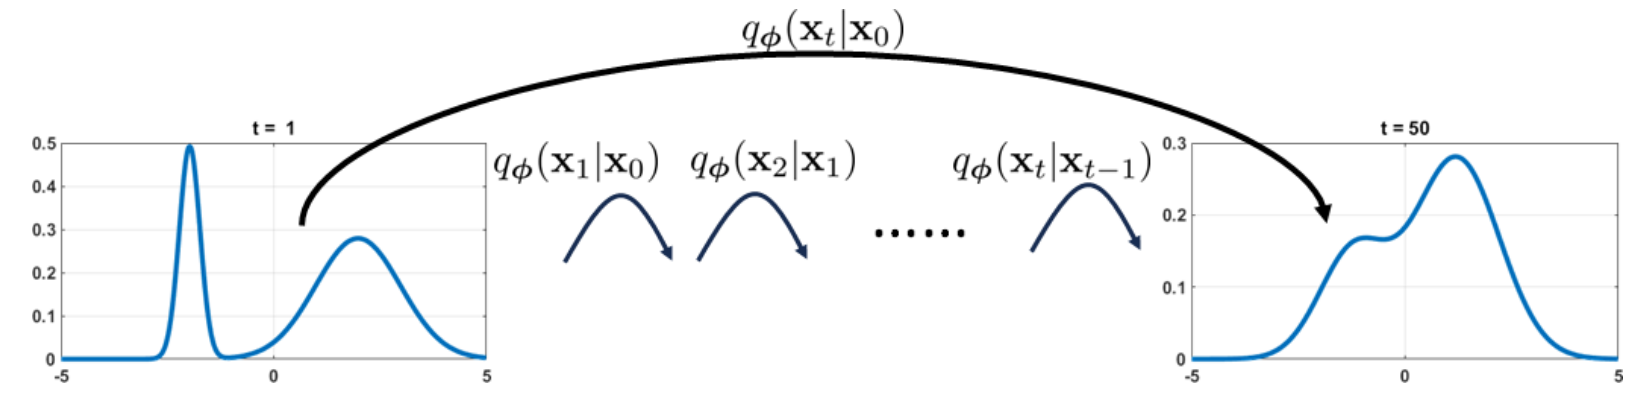
\includegraphics[width=0.8\linewidth]{figs/conditional_diffusion}
	\end{figure}
	\vspace{-0.5cm}
	\begin{block}{Statement 2}
		Applying the Markov chain to any distribution $\pi(\bx)$ yields $\bx_\infty \sim p_\infty(\bx) = \cN(0, \bI)$, the \textbf{stationary} (limiting) distribution:
		\[
			p_\infty(\bx) = \int q(\bx | \bx') p_\infty(\bx') d\bx' 
		\]
		\[
			p_\infty(\bx) = \int q(\bx_\infty | \bx_0) \pi(\bx_0) d\bx_0 \approx \cN(0, \bI) \int \pi(\bx_0) d\bx_0 = \cN(0, \bI)
		\]
		\vspace{-0.8cm}
	\end{block}
	\myfootnote{\href{https://arxiv.org/abs/2403.18103}{Chan S. Tutorial on Diffusion Models for Imaging and Vision, 2024} \\ \href{http://proceedings.mlr.press/v37/sohl-dickstein15.pdf}{Sohl-Dickstein J. Deep Unsupervised Learning using Nonequilibrium Thermodynamics, 2015}}
 \end{frame}
%=======
\begin{frame}{Forward Gaussian Diffusion Process}
	\textbf{Diffusion} describes the migration of particles from regions of high density to those of low density.
	\vspace{-0.2cm}
	\begin{figure}
		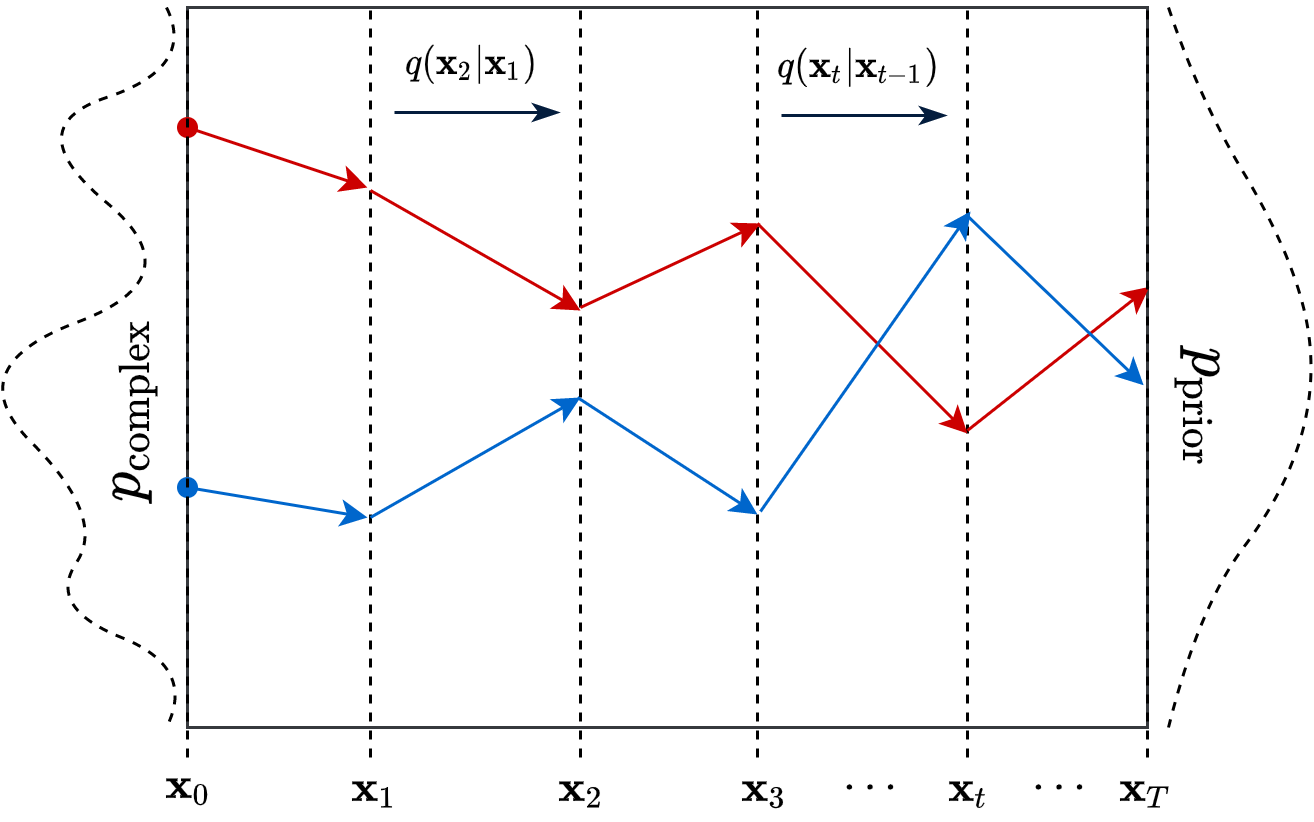
\includegraphics[width=0.5\linewidth]{figs/diffusion_over_time}
	\end{figure}
	\vspace{-0.6cm}
	\begin{enumerate}
		\item $\bx_0 = \bx \sim \pi(\bx)$
		\item $\bx_t = \sqrt{1 - \beta_t} \bx_{t-1} + \sqrt{\beta_t} \bepsilon$, $\bepsilon \sim \cN(0, \bI)$, $t \geq 1$
		\item After $T \gg 1$ steps: $\bx_T \sim p_\infty(\bx) = \cN(0, \bI)$
	\end{enumerate}
	If this process can be reversed, we can sample from $\pi(\bx)$ by starting from noise $p_\infty(\bx) = \cN(0, \bI)$. \\
	Our goal now becomes inverting this diffusion.
	\myfootnotewithlink{https://ayandas.me/blog-tut/2021/12/04/diffusion-prob-models.html}{Das A. An introduction to Diffusion Probabilistic Models, blog post, 2021}
\end{frame}
%=======
\section{Denoising Score Matching for Diffusion}
%=======
\begin{frame}{Denoising Score Matching}
	\begin{block}{NCSN} 
		\vspace{-0.7cm} 
		\[
			q(\bx_t | \bx_0) = \cN(\bx_0, \sigma_t^2 \bI), \quad q(\bx_1) \approx \pi(\bx), \quad q(\bx_T) \approx \cN(0, \sigma_T^2 \bI)
		\]
		\[
			\nabla_{\bx_t} \log q(\bx_t | \bx) = - \frac{\bx_t - \bx}{\sigma_t^2}
		\]
		\vspace{-0.6cm} 
	\end{block}
	\begin{block}{Gaussian Diffusion}
		\vspace{-0.7cm} 
		\[
			q(\bx_t | \bx_0) = \cN(\sqrt{\bar{\alpha}_t} \bx_0, (1 - \bar{\alpha}_t) \bI), \quad q(\bx_1) \approx \pi(\bx), \quad q(\bx_T) \approx \cN(0, \bI)
		\]
		\[
			\nabla_{\bx_t} \log q(\bx_t | \bx_0) = - \frac{\bx_t - \sqrt{\bar{\alpha}_t} \bx_0}{1 - \bar{\alpha}_t}
		\]
		\vspace{-0.6cm} 
	\end{block}
	\begin{block}{Theorem (Denoising Score Matching)}
	\vspace{-0.7cm}
	\begin{multline*}
		\bbE_{q(\bx_t)}\left\| \bs_{\btheta, t}(\bx_t) - \nabla_{\bx_t} \log q(\bx_t) \right\|_2^2 = \\
		= \bbE_{\pi(\bx)} \bbE_{q(\bx_t | \bx)}\left\| \bs_{\btheta, t}(\bx_t) - \nabla_{\bx_t} \log q(\bx_t | \bx) \right\|_2^2 + \text{const}(\btheta)
	\end{multline*}
	\vspace{-0.5cm}
	\end{block}
	\textbf{Note:} This enables applying the NCSN approach with annealed Langevin dynamics to diffusion-based denoising models.
\end{frame}
%=======
\section{Reverse Gaussian Diffusion Process}
%=======
\begin{frame}{Reverse Gaussian Diffusion Process}
	\begin{figure}
		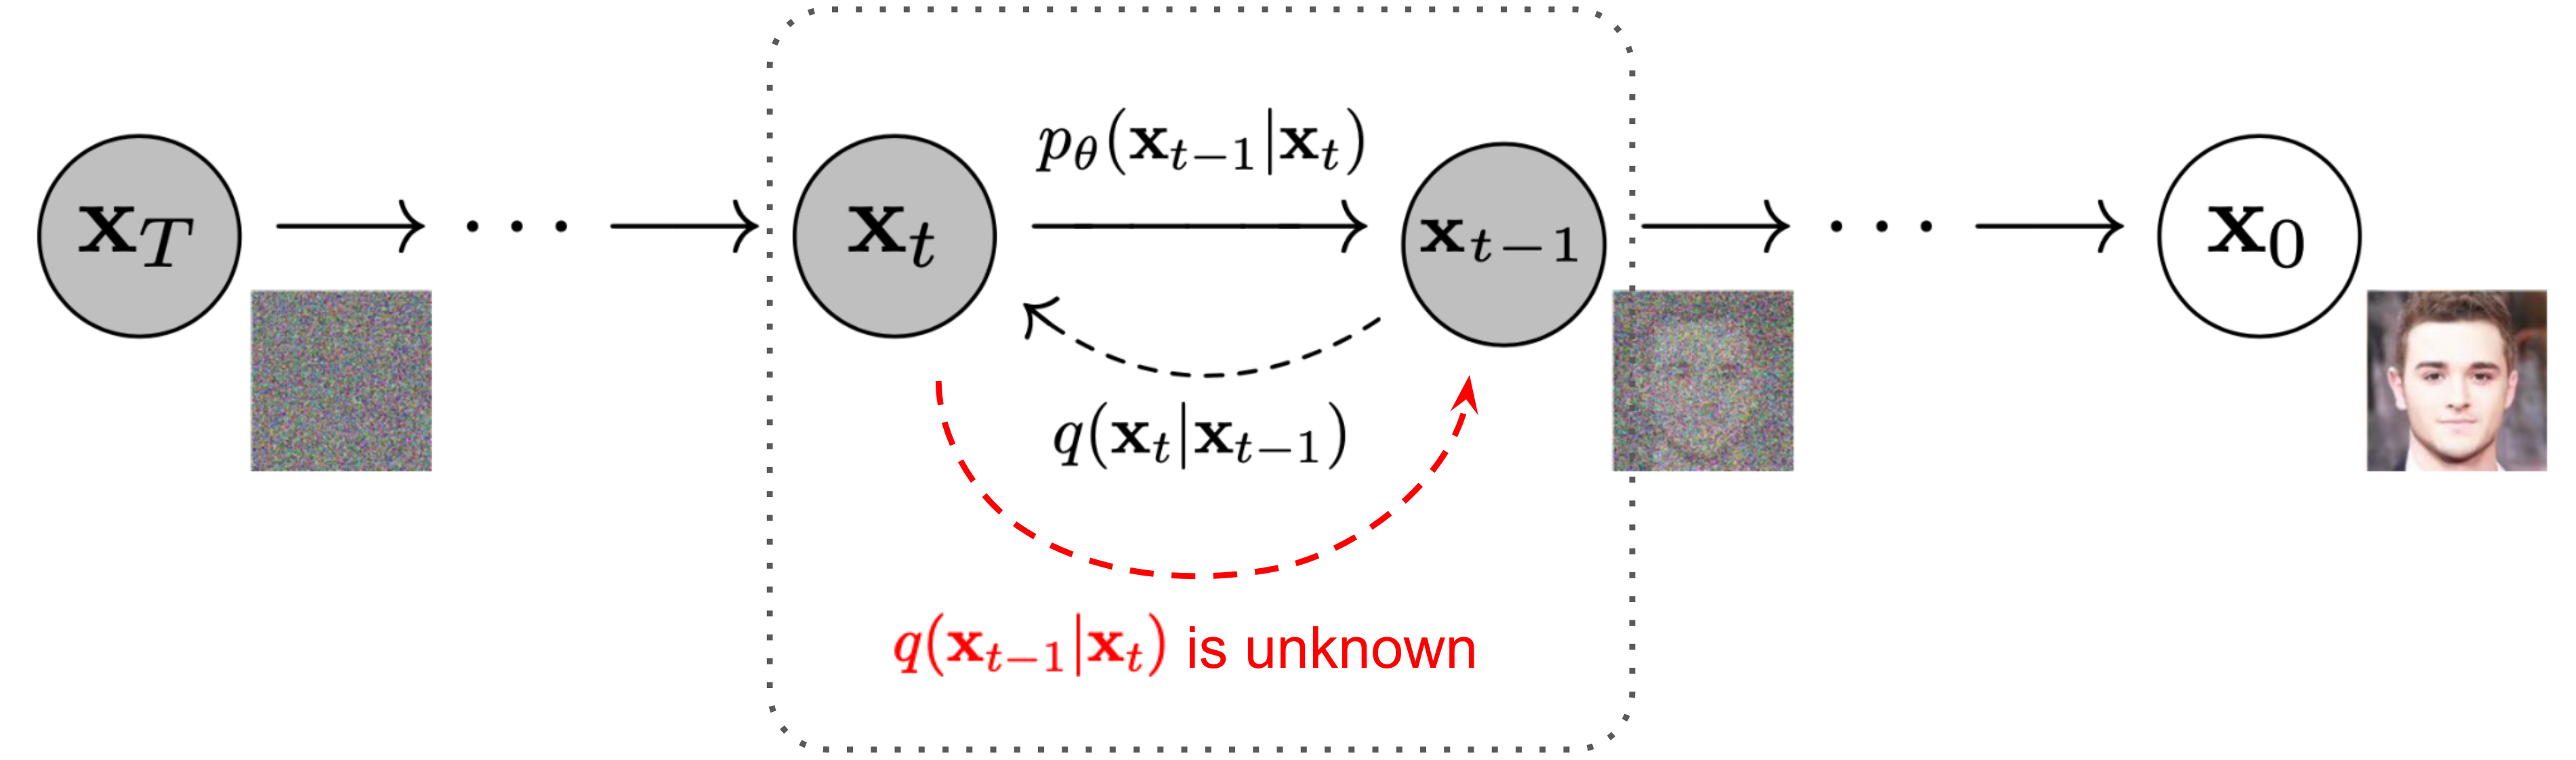
\includegraphics[width=0.8\linewidth]{figs/DDPM}
	\end{figure}
	\vspace{-0.5cm}
	\begin{block}{Forward Process}
		\vspace{-0.3cm}
		\[
			q(\bx_t | \bx_{t-1}) = \cN\left(\sqrt{1 - \beta_t} \bx_{t-1}, \beta_t \bI\right)
		\]
		\vspace{-0.5cm}
	\end{block}
	\begin{block}{Reverse Process}
		\vspace{-0.3cm}
		\[
			q(\bx_{t-1}\mid\bx_{t}) = \frac{q(\bx_{t}\mid\bx_{t-1}) {\color{violet}q(\bx_{t-1})}}{{\color{violet}q(\bx_{t})}} \approx p(\bx_{t - 1} | \bx_t, \btheta)
		\]
		\vspace{-0.3cm}
		${\color{violet}q(\bx_{t-1})}$ and ${\color{violet}q(\bx_{t})}$ are intractable:
		\[
			q(\bx_{t}) = \int q(\bx_{t} | \bx_0) \pi(\bx_0) d\bx_0
		\]
	\end{block}
	\myfootnotewithlink{https://lilianweng.github.io/posts/2021-07-11-diffusion-models/}{Weng L. What are Diffusion Models?, blog post, 2021}
\end{frame}
%=======
\begin{frame}{Reverse Gaussian Diffusion Process}
		\vspace{-0.4cm}
		\[
			q(\bx_{t-1}|\bx_{t}) = \frac{q(\bx_{t}|\bx_{t-1}) {\color{violet}q(\bx_{t-1})}}{{\color{violet}q(\bx_{t})}} 
		\]
		\vspace{-0.4cm}
		\begin{block}{Theorem (Feller, 1949)}
			If $\beta_t$ is sufficiently small, $q(\bx_{t-1}|\bx_t)$ is Gaussian {\color{gray}(thus, diffusion requires $T \approx 1000$ steps for convergence)}
		\end{block}
		\vspace{-0.3cm}
		\begin{figure}
			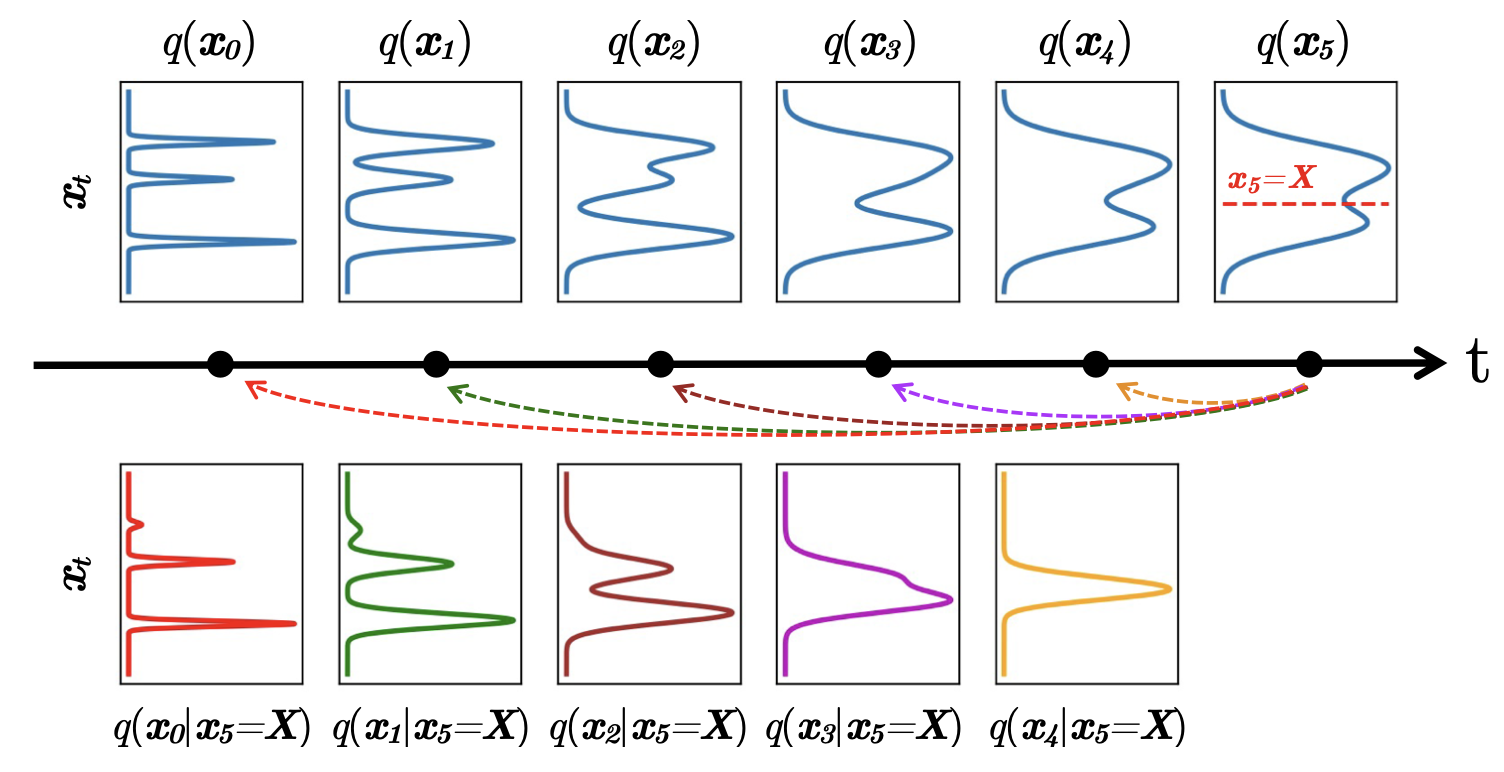
\includegraphics[width=0.7\linewidth]{figs/inverse_distr_1d}
		\end{figure}
	\myfootnote{\href{}{Feller W. On the theory of stochastic processes, with particular reference to applications, 1949} \\ 
	\href{https://arxiv.org/abs/2112.07804}{Xiao Z., Kreis K., Vahdat A. Tackling the generative learning trilemma with denoising diffusion GANs, 2021}}
	\end{frame} 
%=======
\begin{frame}{Reverse Gaussian Diffusion Process (Ancestral Sampling)}
	\vspace{-0.3cm} 
	\begin{figure}
		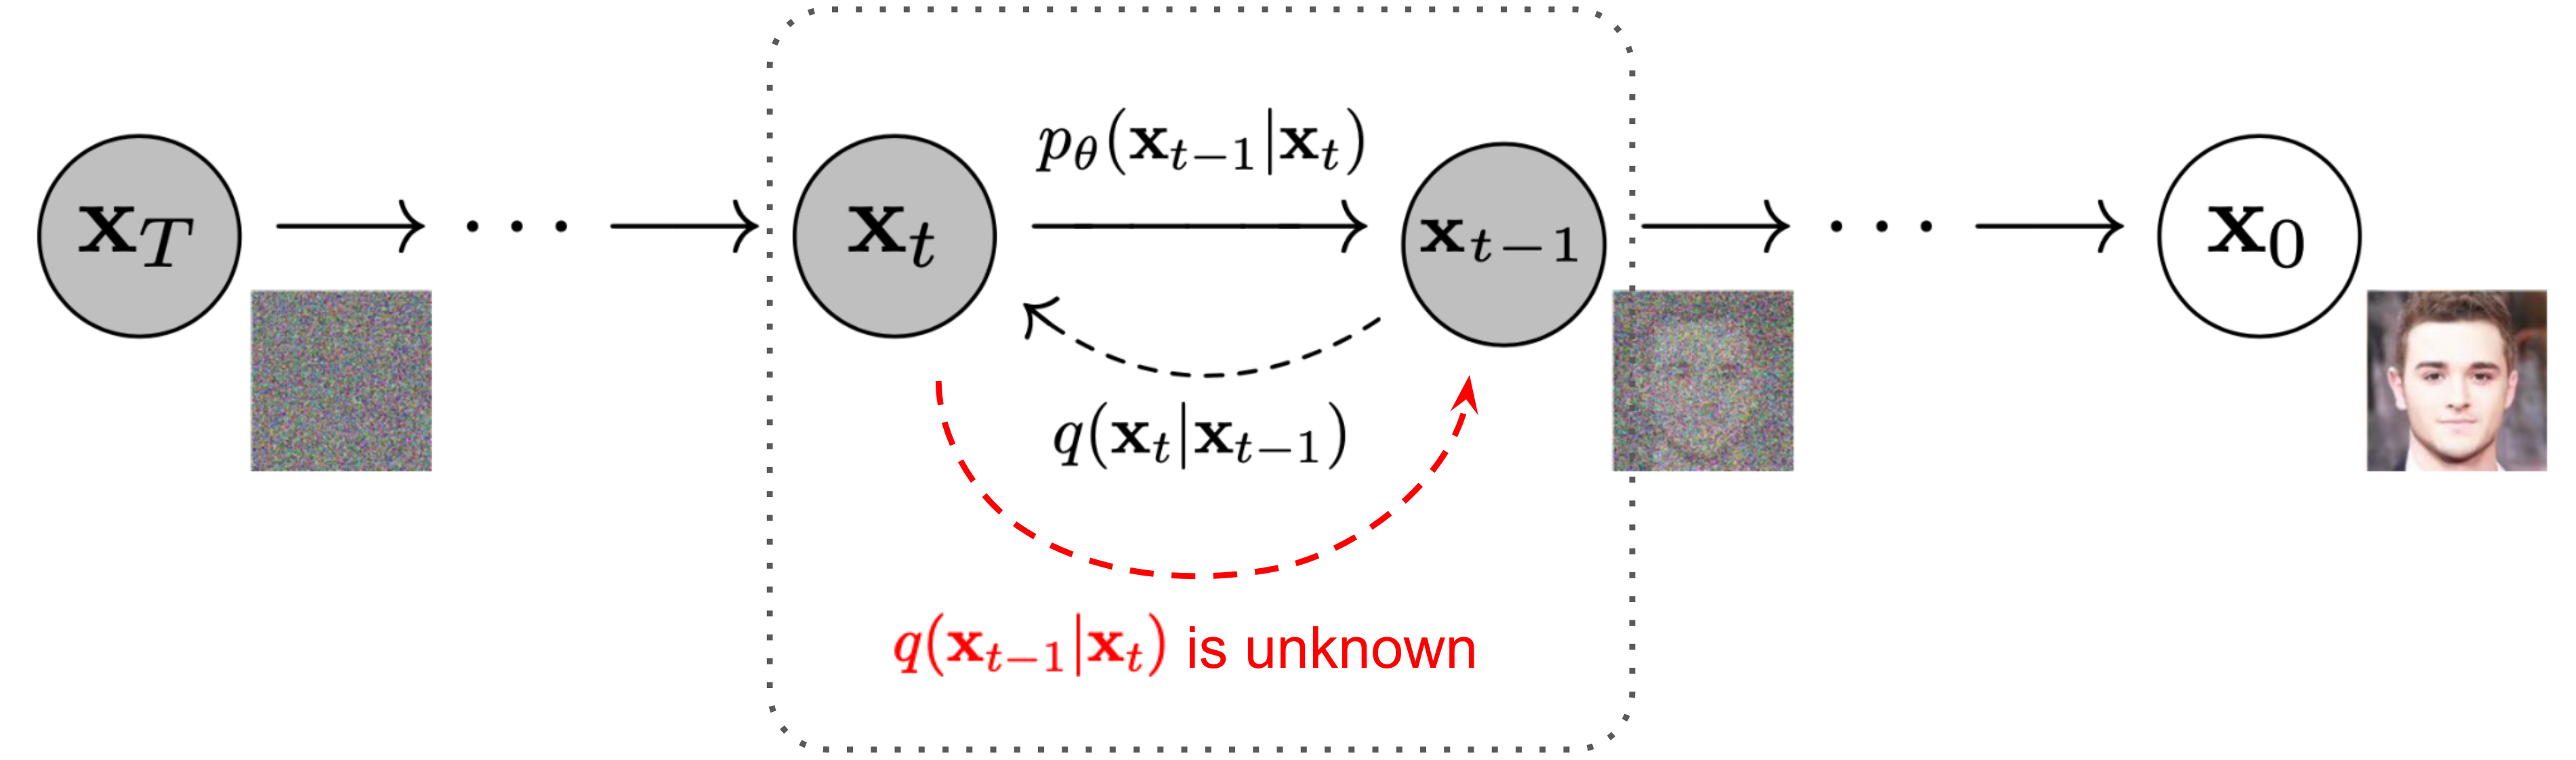
\includegraphics[width=0.8\linewidth]{figs/DDPM}
	\end{figure}
	\vspace{-0.3cm} 
	Define the reverse process as: 
	\vspace{-0.2cm}
	\[
		q(\bx_{t-1}|\bx_{t}) \approx p(\bx_{t - 1} | \bx_t, \btheta) = \cN\bigl(\bmu_{\btheta, t}(\bx_t), \bsigma^2_{\btheta, t}(\bx_t)\bigr)
	\]
	{\color{gray}Feller's theorem justifies this Gaussian assumption.}
	\begin{minipage}{0.5\linewidth}
		\begin{block}{Forward Process}
			\begin{enumerate}
				\item $\bx_0 = \bx \sim \pi(\bx)$
				\item $\bx_t = \sqrt{1 - \beta_t} \bx_{t-1} + \sqrt{\beta_t} \bepsilon$
				\item $\bx_T \sim p_\infty(\bx) = \cN(0, \bI)$
			\end{enumerate}
		\end{block}
	\end{minipage}%
	\begin{minipage}{0.55\linewidth}
		\begin{block}{Reverse Process}
			\begin{enumerate}
				\item $\bx_T \sim p_\infty(\bx) = \cN(0, \bI)$
				\item $\bx_{t-1} = \bsigma_{\btheta, t}(\bx_t) \bepsilon + \bmu_{\btheta, t}(\bx_t)$
				\item $\bx_0 = \bx \sim \pi(\bx)$
			\end{enumerate}
		\end{block}
	\end{minipage}
	\textbf{Note:} The forward process is non-learnable, i.e., it does not involve trainable parameters
	\myfootnotewithlink{https://lilianweng.github.io/posts/2021-07-11-diffusion-models/}{Weng L. What are Diffusion Models?, blog post, 2021}
\end{frame}
%=======
\begin{frame}{Summary}
	\begin{itemize}
		\item Denoising score matching minimizes the Fisher divergence on corrupted samples, making the divergence estimable via sampling
		\vfill 
		\item The noise-conditioned score network leverages a range of noise levels and annealed Langevin dynamics to learn the score function and enable sampling	
		\vfill
		\item The Gaussian diffusion process is a Markov chain that incrementally corrupts data with carefully structured Gaussian noise
		\vfill
		\item Denoising score matching, together with Langevin dynamics, can be applied to the Gaussian diffusion process
		\vfill
		\item The reverse process reconstructs data from noise samples, although its precise form is intractable
	\end{itemize}
\end{frame}
%=======
\end{document}